\documentclass[12pt,a4paper]{report}
\usepackage[margin=1in]{geometry}
\usepackage[T1]{fontenc}
\usepackage[utf8]{inputenc}
\usepackage{lmodern}
\usepackage{setspace}
\usepackage{xurl}
\usepackage{hyperref}
\usepackage{xcolor}
\usepackage{graphicx}
\usepackage{pdflscape}
\usepackage{tikz}
\usepackage{booktabs}
\usepackage{longtable}
\usepackage{array}
\usepackage{enumitem}
\usepackage{listings}
\usepackage{upquote}
\usepackage{caption}
\usepackage{tabularx}
\usepackage{needspace}
\usetikzlibrary{arrows.meta,positioning,shapes.geometric}

\input{glyphtounicode}
\pdfgentounicode=1

\definecolor{codebg}{RGB}{248,248,248}
\definecolor{coderule}{RGB}{220,220,220}
\definecolor{flowblue}{RGB}{232,241,252}
\definecolor{flowgreen}{RGB}{232,247,237}
\definecolor{floworange}{RGB}{255,243,224}
\definecolor{flowred}{RGB}{252,232,232}

\tikzset{
  flowbox/.style={
    rectangle,
    rounded corners=3pt,
    draw=black!55,
    very thick,
    align=center,
    text width=3.1cm,
    minimum height=1.05cm,
    inner sep=6pt,
    font=\small
  },
  flowio/.style={
    trapezium,
    trapezium left angle=70,
    trapezium right angle=110,
    draw=black!55,
    very thick,
    align=center,
    text width=3.0cm,
    minimum height=1.05cm,
    inner sep=6pt,
    font=\small
  },
  flowdecision/.style={
    diamond,
    aspect=2.0,
    draw=black!55,
    very thick,
    align=center,
    text width=2.9cm,
    inner sep=3pt,
    font=\small
  },
  flowarrow/.style={
    -{Latex[length=3mm]},
    very thick,
    draw=black!70
  }
}

\lstdefinestyle{reportcode}{
  basicstyle=\ttfamily\scriptsize,
  backgroundcolor=\color{codebg},
  frame=single,
  rulecolor=\color{coderule},
  breaklines=true,
  breakatwhitespace=false,
  columns=fullflexible,
  keepspaces=true,
  showstringspaces=false,
  upquote=true,
  tabsize=2,
  captionpos=b,
  xleftmargin=0.5em,
  xrightmargin=0.5em,
  numbers=left,
  numberstyle=\tiny,
  numbersep=8pt
}

\lstdefinestyle{terminalcode}{
  style=reportcode,
  numbers=none,
  numbersep=0pt,
  xleftmargin=0.5em
}

\newcommand{\codenext}[1]{\par\Needspace{#1\baselineskip}}
\newcommand{\codepath}[1]{\path{#1}}

\setlist[itemize]{leftmargin=1.2cm}
\setlist[enumerate]{leftmargin=1.2cm}
\setstretch{1.0}
\emergencystretch=4em
\sloppy

\title{MFJA 3rd Floor Gazebo Harmonic\\Current Multi-Robot and Room 315 Kinematic Shuttle Report}
\author{Technical Project Report}
\date{\today}

\begin{document}
\maketitle
\tableofcontents
\clearpage

\chapter{Purpose and Current Scope}

This report documents the current accepted state of the
\texttt{mfja\_3rd\_floor\_gz} meta-repository. The project now combines two
main layers:

\begin{itemize}
\item a reusable Gazebo Harmonic and ROS~2 Jazzy multi-robot simulation for the
MFJA third floor;
\item a kinematic-first Room 315 shuttle simulation for the flexible rail
network.
\end{itemize}

The current shuttle work is intentionally kinematic. The shuttle does not use
wheel contact, rail contact dynamics, or full rigid-body contact as the primary
motion source. Instead, the rail path is represented as CSV geometry plus an
explicit directed graph. The node computes the shuttle pose along rail segments
and sends pose updates to Gazebo through
\texttt{/world/<world\_name>/set\_pose}.

Dynamic shuttle work is not part of the current main version. The current main
version focuses on:

\begin{itemize}
\item independent robot control through namespaced ROS topics;
\item a clean ROS~2 meta-repository package structure;
\item Room 315 kinematic shuttle routing;
\item independent switch states;
\item independent binary stoppers before switches;
\item sensor-style approach events for the teaching workflow;
\item per-shuttle ON/OFF commands;
\item runtime shuttle spawning;
\item explicit rejection when a requested start slot is occupied;
\item simple center-distance collision avoidance between shuttles.
\end{itemize}

\begin{figure}[p]
\centering
\resizebox{0.95\textwidth}{!}{%
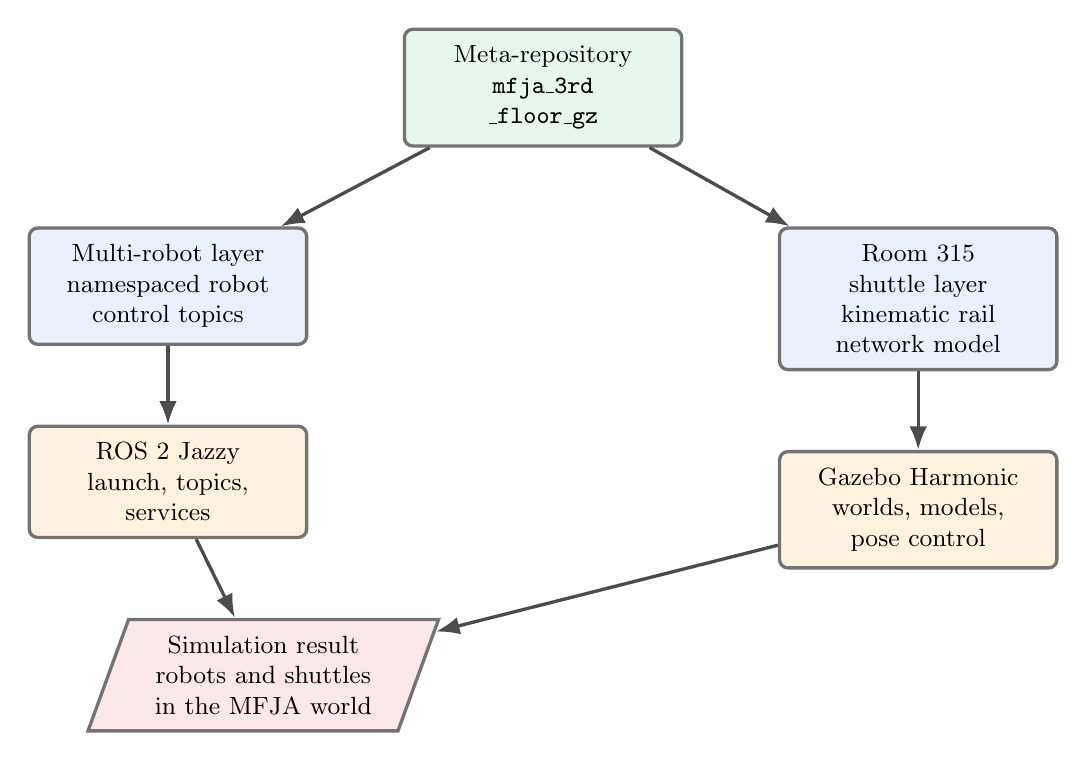
\begin{tikzpicture}[node distance=1.0cm and 1.2cm]
\node[flowbox, fill=flowgreen] (repo) {Meta-repository\\\texttt{mfja\_3rd}\\\texttt{\_floor\_gz}};
\node[flowbox, fill=flowblue, below left=of repo] (robots) {Multi-robot layer\\namespaced robot\\control topics};
\node[flowbox, fill=flowblue, below right=of repo] (shuttle) {Room 315 shuttle layer\\kinematic rail\\network model};
\node[flowbox, fill=floworange, below=of robots] (ros) {ROS 2 Jazzy\\launch, topics,\\services};
\node[flowbox, fill=floworange, below=of shuttle] (gz) {Gazebo Harmonic\\worlds, models,\\pose control};
\node[flowio, fill=flowred, below right=1.0cm and -1.3cm of ros] (demo) {Simulation result\\robots and shuttles\\in the MFJA world};

\draw[flowarrow] (repo) -- (robots);
\draw[flowarrow] (repo) -- (shuttle);
\draw[flowarrow] (robots) -- (ros);
\draw[flowarrow] (shuttle) -- (gz);
\draw[flowarrow] (ros) -- (demo);
\draw[flowarrow] (gz) -- (demo);
\end{tikzpicture}}
\caption{High-level project scope. The repository now contains a general
multi-robot simulation layer and a Room 315 kinematic shuttle layer. Both are
integrated through ROS 2 and Gazebo.}
\label{fig:project-scope-flow}
\end{figure}

\chapter{Repository Architecture}

\section{Meta-repository layout}

The Git repository root is intentionally not a ROS~2 package. The root contains
documentation and repository-level files only. ROS packages live in subfolders:

\begin{itemize}
\item \texttt{mfja\_3rd\_floor\_description}: shared Gazebo models, meshes,
worlds, and URDF/SDF assets;
\item \texttt{mfja\_robot\_control\_config}: shared launch logic, bridge
configuration, robot registries, Room 315 kinematic configuration, and control
scripts;
\item \texttt{mfja\_room\_315\_bringup}: launch entry point for Room 315 only;
\item \texttt{mfja\_3rd\_floor\_bringup}: launch entry point for the full
floor;
\item \texttt{mfja\_3rd\_floor\_gz}: umbrella compatibility package that keeps
historical launch entry points available.
\end{itemize}

The root should not contain package-level files such as root
\texttt{package.xml}, root \texttt{CMakeLists.txt}, root \texttt{models/},
root \texttt{worlds/}, root \texttt{launch/}, root \texttt{config/}, or root
\texttt{CSV/}. Package-owned files belong inside the package that owns them.

\begin{figure}[p]
\centering
\resizebox{\textwidth}{!}{%
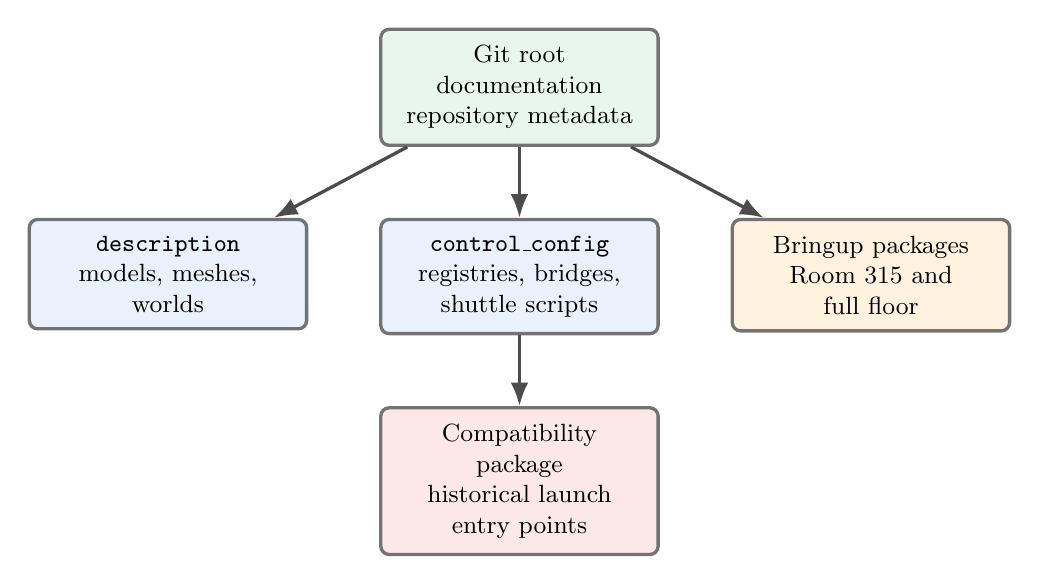
\begin{tikzpicture}[node distance=0.9cm and 0.9cm]
\node[flowbox, fill=flowgreen] (root) {Git root\\documentation\\repository metadata};
\node[flowbox, fill=flowblue, below left=of root] (desc) {\texttt{description}\\models, meshes,\\worlds};
\node[flowbox, fill=flowblue, below=of root] (control) {\texttt{control\_config}\\registries, bridges,\\shuttle scripts};
\node[flowbox, fill=floworange, below right=of root] (bringups) {Bringup packages\\Room 315 and\\full floor};
\node[flowbox, fill=flowred, below=of control] (compat) {Compatibility package\\historical launch\\entry points};

\draw[flowarrow] (root) -- (desc);
\draw[flowarrow] (root) -- (control);
\draw[flowarrow] (root) -- (bringups);
\draw[flowarrow] (control) -- (compat);
\end{tikzpicture}}
\caption{Repository ownership model. The root is not a ROS 2 package. Runtime
assets live inside the package that owns them, which keeps the workspace
buildable and easier to maintain.}
\label{fig:repo-architecture-flow}
\end{figure}

\section{Build command}

The explicit \texttt{--base-paths} command is the recommended build method,
because the repository contains several ROS~2 packages inside one Git
repository.

\codenext{18}
\begin{lstlisting}[style=terminalcode,caption={Current meta-repository build command.}]
cd /home/tiago/ALI_ros2_ws
source /opt/ros/jazzy/setup.bash

colcon build --base-paths \
  src/mfja_3rd_floor_gz/mfja_robot_control_config \
  src/mfja_3rd_floor_gz/mfja_3rd_floor_description \
  src/mfja_3rd_floor_gz/mfja_room_315_bringup \
  src/mfja_3rd_floor_gz/mfja_3rd_floor_bringup \
  src/mfja_3rd_floor_gz/mfja_3rd_floor_gz \
  --packages-select \
  mfja_robot_control_config \
  mfja_3rd_floor_description \
  mfja_room_315_bringup \
  mfja_3rd_floor_bringup \
  mfja_3rd_floor_gz \
  --symlink-install

source install/setup.bash
\end{lstlisting}

\chapter{Multi-Robot Simulation Layer}

\section{Supported robots}

The current simulation supports these robot instances:

\begingroup
\small
\begin{longtable}{@{}p{0.24\textwidth}p{0.18\textwidth}p{0.44\textwidth}@{}}
\toprule
Instance & Robot family & Primary command topic \\
\midrule
\endhead
\texttt{kuka1} & KUKA KR6 R900 sixx & \texttt{/kuka1/joint\_trajectory} \\
\texttt{staubli1} & Staeubli TX2-60L & \texttt{/staubli1/joint\_trajectory} \\
\texttt{yaskawa\_hc10\_1} & Yaskawa HC10 & \texttt{/yaskawa\_hc10\_1/joint\_trajectory} \\
\texttt{yaskawa\_hc10dt\_1} & Yaskawa HC10DT & \texttt{/yaskawa\_hc10dt\_1/joint\_trajectory} \\
\texttt{tiago1} & TIAGo mobile manipulator & \texttt{/tiago1/joint\_trajectory}, \texttt{/tiago1/cmd\_vel} \\
\bottomrule
\end{longtable}
\endgroup

Each robot uses its own namespace. A command sent to one namespace does not
affect another robot.

\begin{landscape}
\begin{figure}[p]
\centering
\resizebox{0.96\linewidth}{!}{%
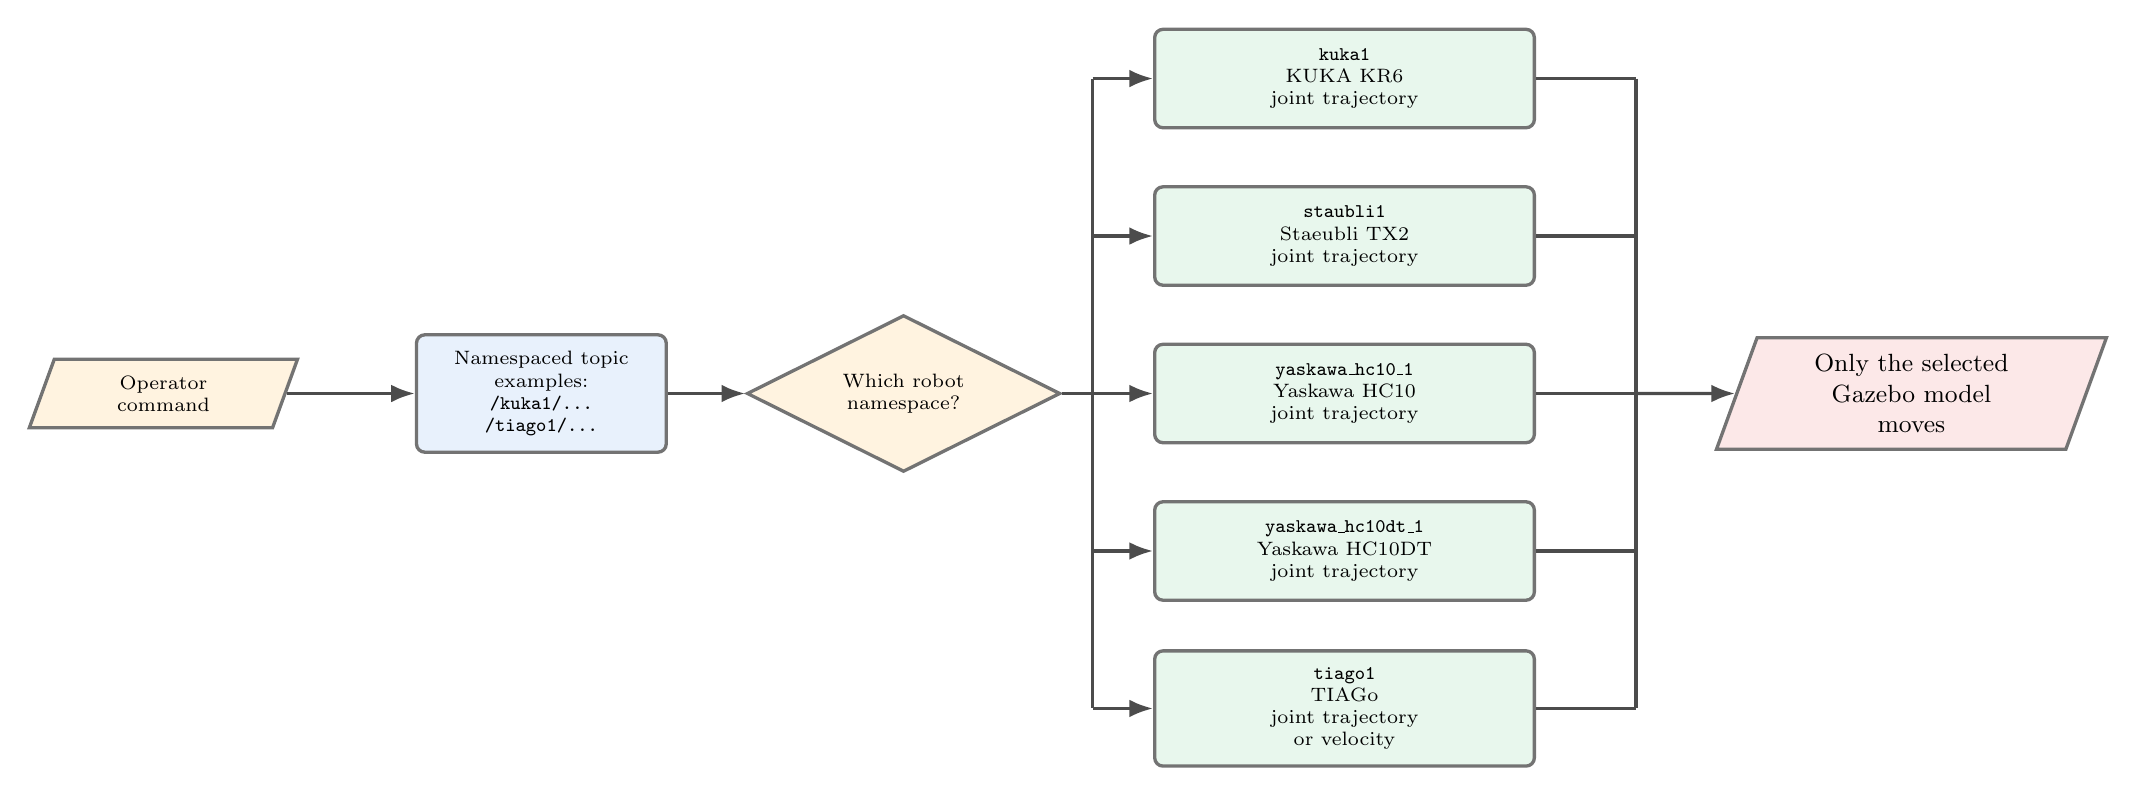
\begin{tikzpicture}[node distance=0.9cm and 0.9cm]
\tikzset{
  robotbox/.style={
    rectangle,
    rounded corners=3pt,
    draw=black!55,
    very thick,
    align=center,
    text width=4.4cm,
    minimum height=1.25cm,
    inner sep=6pt,
    font=\scriptsize,
    fill=flowgreen
  }
}
\node[flowio, fill=floworange, text width=2.35cm, minimum height=0.85cm, font=\scriptsize] (operator) at (0,0) {Operator\\command};
\node[flowbox, fill=flowblue, text width=2.75cm, minimum height=0.95cm, font=\scriptsize] (topic) at (4.8,0) {Namespaced topic\\examples:\\\texttt{/kuka1/...}\\\texttt{/tiago1/...}};
\node[flowdecision, fill=floworange, text width=2.35cm, font=\scriptsize] (ns) at (9.4,0) {Which robot\\namespace?};

\node[robotbox] (kuka) at (15.0,4.0) {\texttt{kuka1}\\KUKA KR6\\joint trajectory};
\node[robotbox] (staubli) at (15.0,2.0) {\texttt{staubli1}\\Staeubli TX2\\joint trajectory};
\node[robotbox] (hc10) at (15.0,0.0) {\texttt{yaskawa\_hc10\_1}\\Yaskawa HC10\\joint trajectory};
\node[robotbox] (hc10dt) at (15.0,-2.0) {\texttt{yaskawa\_hc10dt\_1}\\Yaskawa HC10DT\\joint trajectory};
\node[robotbox] (tiago) at (15.0,-4.0) {\texttt{tiago1}\\TIAGo\\joint trajectory\\or velocity};

\node[flowio, fill=flowred, text width=3.5cm] (gazebo) at (22.2,0) {Only the selected\\Gazebo model\\moves};

\coordinate (split) at (11.8,0);
\coordinate (splitkuka) at (11.8,4.0);
\coordinate (splitstaubli) at (11.8,2.0);
\coordinate (splithc10) at (11.8,0.0);
\coordinate (splithc10dt) at (11.8,-2.0);
\coordinate (splittiago) at (11.8,-4.0);

\coordinate (join) at (18.7,0);
\coordinate (joinkuka) at (18.7,4.0);
\coordinate (joinstaubli) at (18.7,2.0);
\coordinate (joinhc10) at (18.7,0.0);
\coordinate (joinhc10dt) at (18.7,-2.0);
\coordinate (jointiago) at (18.7,-4.0);

\draw[flowarrow] (operator.east) -- (topic.west);
\draw[flowarrow] (topic.east) -- (ns.west);
\draw[very thick, draw=black!70] (ns.east) -- (split);
\draw[very thick, draw=black!70] (splitkuka) -- (splittiago);
\draw[flowarrow] (splitkuka) -- (kuka.west);
\draw[flowarrow] (splitstaubli) -- (staubli.west);
\draw[flowarrow] (splithc10) -- (hc10.west);
\draw[flowarrow] (splithc10dt) -- (hc10dt.west);
\draw[flowarrow] (splittiago) -- (tiago.west);

\draw[very thick, draw=black!70] (joinkuka) -- (jointiago);
\draw[very thick, draw=black!70] (kuka.east) -- (joinkuka);
\draw[very thick, draw=black!70] (staubli.east) -- (joinstaubli);
\draw[very thick, draw=black!70] (hc10.east) -- (joinhc10);
\draw[very thick, draw=black!70] (hc10dt.east) -- (joinhc10dt);
\draw[very thick, draw=black!70] (tiago.east) -- (jointiago);
\draw[flowarrow] (join) -- (gazebo.west);
\end{tikzpicture}}
\caption{Namespaced robot control for all supported robot instances. Each
command is routed through one robot namespace, so commanding one robot does not
move the others.}
\label{fig:robot-namespace-flow}
\end{figure}
\end{landscape}

\section{Robot registries}

Robot identity, model selection, pose, and activation are stored in YAML
registries:

\begin{itemize}
\item \codepath{mfja_robot_control_config/config/robots.yaml} for the full
floor;
\item \codepath{mfja_robot_control_config/config/robots_room_315_only.yaml}
for Room 315 only.
\end{itemize}

This makes robot deployment data-driven. A developer can adjust active robots
and placements without editing the launch implementation.

\section{Full floor launch}

\codenext{10}
\begin{lstlisting}[style=terminalcode,caption={Launching the full floor.}]
cd /home/tiago/ALI_ros2_ws
source /opt/ros/jazzy/setup.bash
source install/setup.bash

ros2 launch mfja_3rd_floor_bringup full_floor.launch.py \
  robots:=none \
  start_paused:=false \
  gui:=true
\end{lstlisting}

\section{Room 315 only launch}

\codenext{10}
\begin{lstlisting}[style=terminalcode,caption={Launching Room 315 only.}]
cd /home/tiago/ALI_ros2_ws
source /opt/ros/jazzy/setup.bash
source install/setup.bash

ros2 launch mfja_room_315_bringup room_315_only.launch.py \
  robots:=none \
  start_paused:=false \
  gui:=true
\end{lstlisting}

\section{Robot topic checks}

\codenext{10}
\begin{lstlisting}[style=terminalcode,caption={Checking robot control topics.}]
ros2 topic list | grep -E '^/(kuka1|staubli1|yaskawa_hc10_1|yaskawa_hc10dt_1|tiago1)/'

ros2 topic info /kuka1/joint_trajectory
ros2 topic info /staubli1/joint_trajectory
ros2 topic info /yaskawa_hc10_1/joint_trajectory
ros2 topic info /yaskawa_hc10dt_1/joint_trajectory
ros2 topic info /tiago1/joint_trajectory
ros2 topic info /tiago1/cmd_vel
\end{lstlisting}

\section{Example one-robot commands}

\codenext{12}
\begin{lstlisting}[style=terminalcode,caption={KUKA example command.}]
ros2 topic pub --once /kuka1/joint_trajectory \
trajectory_msgs/msg/JointTrajectory \
"{joint_names: ['joint_a1','joint_a2','joint_a3','joint_a4','joint_a5','joint_a6'], \
points: [{positions: [0.6,-1.0,1.1,0.0,0.6,0.0], \
time_from_start: {sec: 3, nanosec: 0}}]}"
\end{lstlisting}

\codenext{12}
\begin{lstlisting}[style=terminalcode,caption={Staeubli example command.}]
ros2 topic pub --once /staubli1/joint_trajectory \
trajectory_msgs/msg/JointTrajectory \
"{joint_names: ['joint_1','joint_2','joint_3','joint_4','joint_5','joint_6'], \
points: [{positions: [0.1,0.4,-0.6,0.0,0.5,0.0], \
time_from_start: {sec: 3, nanosec: 0}}]}"
\end{lstlisting}

\codenext{12}
\begin{lstlisting}[style=terminalcode,caption={TIAGo base example command.}]
ros2 topic pub -r 20 /tiago1/cmd_vel geometry_msgs/msg/Twist \
"{linear: {x: 0.15, y: 0.0, z: 0.0}, angular: {x: 0.0, y: 0.0, z: 0.20}}"
\end{lstlisting}

\section{Synchronized multi-robot tool}

The script \texttt{multi\_robot\_sync\_demo.py} can publish coordinated commands
from one ROS~2 process. It is better than starting several shell commands
manually when multiple robots should begin a scenario together.

\codenext{8}
\begin{lstlisting}[style=terminalcode,caption={Inspecting supported synchronized joints.}]
cd /home/tiago/ALI_ros2_ws
source /opt/ros/jazzy/setup.bash
source install/setup.bash

ros2 run mfja_robot_control_config multi_robot_sync_demo.py --list-joints
\end{lstlisting}

\codenext{10}
\begin{lstlisting}[style=terminalcode,caption={Coordinated motion for selected robots.}]
ros2 run mfja_robot_control_config multi_robot_sync_demo.py \
  --goal kuka1=1.2,-1.2,1.4,0.0,0.3,0.0 \
  --goal staubli1=0.1,0.4,-0.6,0.0,0.5,0.0 \
  --trajectory-duration 4.0
\end{lstlisting}

\chapter{Room 315 Kinematic Shuttle Layer}

\section{Rail network model}

The Room 315 rail system is modeled as a directed graph. CSV files contain the
geometry of each one-way segment. The topology and routing rules are stored in:

\begin{center}
\texttt{mfja\_robot\_control\_config/config/room\_315\_kinematics/rail\_network.yaml}
\end{center}

The source rail segments are stored in:

\begin{center}
\texttt{mfja\_robot\_control\_config/config/room\_315\_kinematics/raw\_segments/}
\end{center}

Every segment is traversed forward only, from CSV \texttt{index=0} to the last
row. Routing is not inferred from exact endpoint equality. Routing is decided
by explicit tables in \texttt{rail\_network.yaml}. If the shuttle reaches a
segment end and no valid successor exists, it enters \texttt{FALLING} mode
instead of teleporting or silently correcting the route.

\section{Current start slots}

Only four start slots are currently accepted:

\begin{longtable}{@{}lll@{}}
\toprule
Slot & Gazebo pose & Notes \\
\midrule
\endhead
\texttt{1} & \texttt{-14.95 -3.86 0.84 0 0 3.14} & upper rail \\
\texttt{2} & \texttt{-15.43 -3.86 0.84 0 0 3.14} & upper rail \\
\texttt{3} & \texttt{-15.24 -5.54 0.84 0 0 0} & lower rail \\
\texttt{4} & \texttt{-14.77 -5.54 0.84 0 0 0} & lower rail \\
\bottomrule
\end{longtable}

Runtime add commands are rejected if the selected start slot is occupied.
This is different from collision avoidance: the shuttle is not created at all
when the requested start slot is blocked.

\begin{figure}[p]
\centering
\resizebox{0.90\textwidth}{!}{%
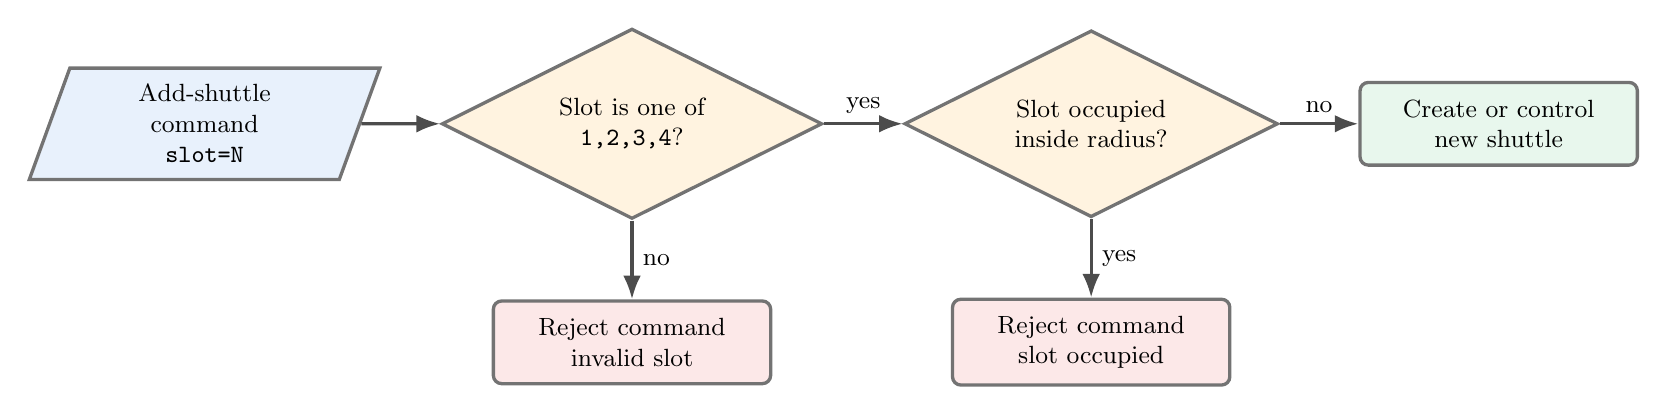
\begin{tikzpicture}[node distance=1.0cm and 1.0cm]
\node[flowio, fill=flowblue] (cmd) {Add-shuttle command\\\texttt{slot=N}};
\node[flowdecision, fill=floworange, right=of cmd] (valid) {Slot is one of\\\texttt{1,2,3,4}?};
\node[flowdecision, fill=floworange, right=of valid] (occupied) {Slot occupied\\inside radius?};
\node[flowbox, fill=flowgreen, right=of occupied] (spawn) {Create or control\\new shuttle};
\node[flowbox, fill=flowred, below=of valid] (badslot) {Reject command\\invalid slot};
\node[flowbox, fill=flowred, below=of occupied] (blocked) {Reject command\\slot occupied};

\draw[flowarrow] (cmd) -- (valid);
\draw[flowarrow] (valid) -- node[above, font=\small] {yes} (occupied);
\draw[flowarrow] (valid) -- node[right, font=\small] {no} (badslot);
\draw[flowarrow] (occupied) -- node[above, font=\small] {no} (spawn);
\draw[flowarrow] (occupied) -- node[right, font=\small] {yes} (blocked);
\end{tikzpicture}}
\caption{Start-slot acceptance logic. A shuttle is added only when the requested
slot exists and the start position is clear.}
\label{fig:start-slot-decision-flow}
\end{figure}

\section{Starting the shuttle node}

The same node works in Room 315 only and in the full floor. The key parameter
is \texttt{gazebo\_world\_name}.

\codenext{12}
\begin{lstlisting}[style=terminalcode,caption={Starting four shuttles in Room 315 only.}]
cd /home/tiago/ALI_ros2_ws
source /opt/ros/jazzy/setup.bash
source install/setup.bash

ros2 run mfja_robot_control_config room_315_kinematic_shuttle_node.py --ros-args \
  -p gazebo_world_name:=room_315_only \
  -p shuttle_count:=4 \
  -p start_slots:=1,2,3,4 \
  -p enable_gazebo_set_pose:=true \
  -p enable_gazebo_spawn:=true \
  -p speed:=0.2 \
  -p gazebo_set_pose_rate_hz:=10.0
\end{lstlisting}

\codenext{12}
\begin{lstlisting}[style=terminalcode,caption={Starting the same shuttle node in the full floor.}]
ros2 run mfja_robot_control_config room_315_kinematic_shuttle_node.py --ros-args \
  -p gazebo_world_name:=mfja_3rd_floor \
  -p shuttle_count:=4 \
  -p start_slots:=1,2,3,4 \
  -p enable_gazebo_set_pose:=true \
  -p enable_gazebo_spawn:=true \
  -p speed:=0.2 \
  -p gazebo_set_pose_rate_hz:=10.0
\end{lstlisting}

\begin{figure}[p]
\centering
\resizebox{0.92\textwidth}{!}{%
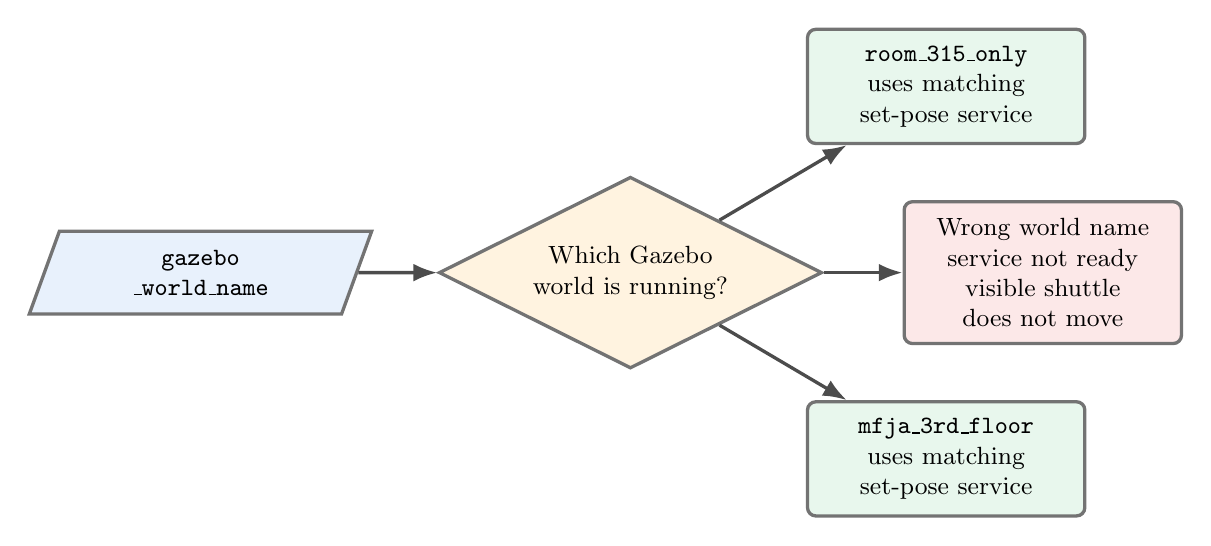
\begin{tikzpicture}[node distance=1.0cm and 1.0cm]
\node[flowio, fill=flowblue] (param) {\texttt{gazebo}\\\texttt{\_world\_name}};
\node[flowdecision, fill=floworange, right=of param] (world) {Which Gazebo\\world is running?};
\node[flowbox, fill=flowgreen, above right=of world] (room) {\texttt{room\_315\_only}\\uses matching\\set-pose service};
\node[flowbox, fill=flowgreen, below right=of world] (floor) {\texttt{mfja\_3rd\_floor}\\uses matching\\set-pose service};
\node[flowbox, fill=flowred, right=of world] (warn) {Wrong world name\\service not ready\\visible shuttle does not move};

\draw[flowarrow] (param) -- (world);
\draw[flowarrow] (world) -- (room);
\draw[flowarrow] (world) -- (floor);
\draw[flowarrow] (world) -- (warn);
\end{tikzpicture}}
\caption{Gazebo world-name selection. The shuttle node can publish ROS topics
without Gazebo moving anything if the set-pose service name does not match the
running world.}
\label{fig:gazebo-world-flow}
\end{figure}

\section{Switch primitive}

Switch routing is controlled by:

\begin{center}
\texttt{/room\_315/switch\_states}
\end{center}

The switch primitive has two logical states:

\begin{itemize}
\item \texttt{G}: big-loop branch;
\item \texttt{S}: small-loop branch.
\end{itemize}

Aliases such as \texttt{BIG}, \texttt{LARGE}, and \texttt{SMALL} are also
accepted by the command layer.

\codenext{8}
\begin{lstlisting}[style=terminalcode,caption={Switch commands.}]
ros2 topic pub --once /room_315/switch_states std_msgs/msg/String "{data: 'ALL=G'}"
ros2 topic pub --once /room_315/switch_states std_msgs/msg/String "{data: 'ALL=S'}"
ros2 topic pub --once /room_315/switch_states std_msgs/msg/String "{data: 'A1=G A2=S A3=G A4=S'}"
\end{lstlisting}

\begin{figure}[p]
\centering
\resizebox{0.95\textwidth}{!}{%
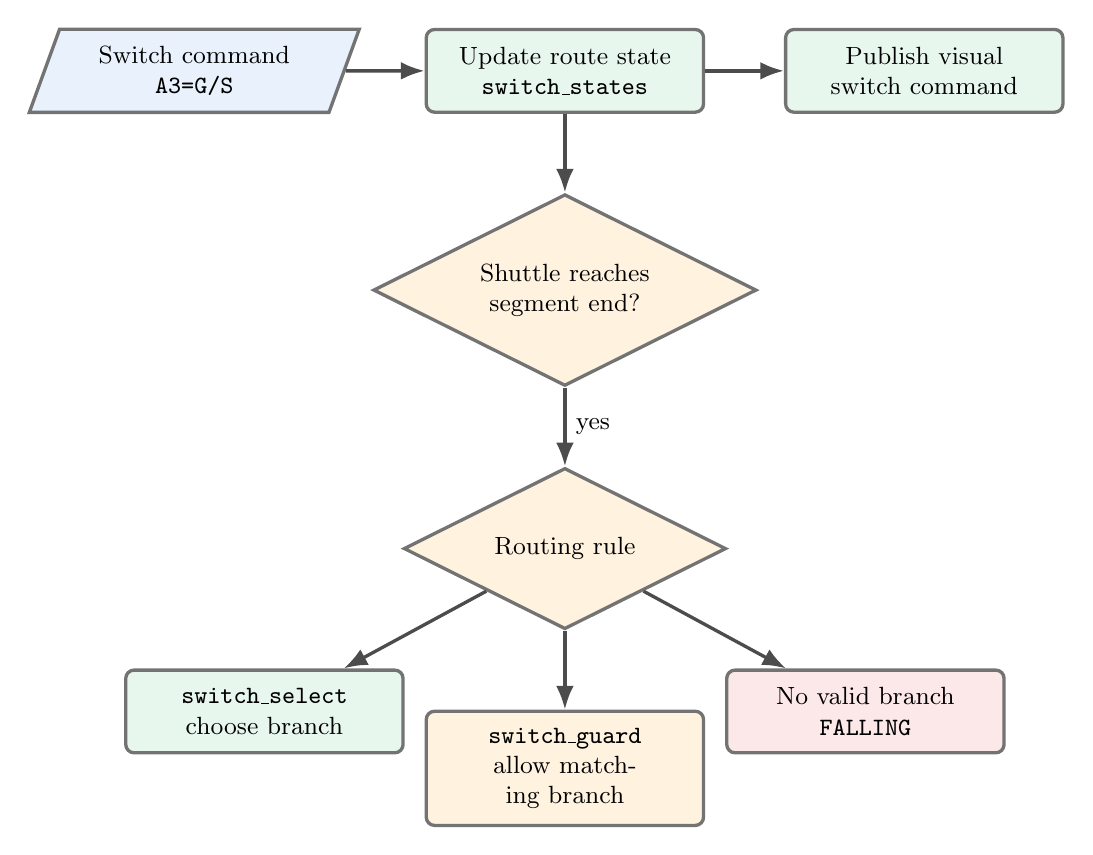
\begin{tikzpicture}[node distance=1.0cm and 1.0cm]
\node[flowio, fill=flowblue] (cmd) {Switch command\\\texttt{A3=G/S}};
\node[flowbox, fill=flowgreen, right=of cmd] (state) {Update route state\\\texttt{switch\_states}};
\node[flowbox, fill=flowgreen, right=of state] (visual) {Publish visual\\switch command};
\node[flowdecision, fill=floworange, below=of state] (end) {Shuttle reaches\\segment end?};
\node[flowdecision, fill=floworange, below=of end] (kind) {Routing rule};
\node[flowbox, fill=flowgreen, below left=of kind] (select) {\texttt{switch\_select}\\choose branch};
\node[flowbox, fill=floworange, below=of kind] (guard) {\texttt{switch\_guard}\\allow matching branch};
\node[flowbox, fill=flowred, below right=of kind] (falling) {No valid branch\\\texttt{FALLING}};

\draw[flowarrow] (cmd) -- (state);
\draw[flowarrow] (state) -- (visual);
\draw[flowarrow] (state) -- (end);
\draw[flowarrow] (end) -- node[right, font=\small] {yes} (kind);
\draw[flowarrow] (kind) -- (select);
\draw[flowarrow] (kind) -- (guard);
\draw[flowarrow] (kind) -- (falling);
\end{tikzpicture}}
\caption{Switch command flow. The same command updates route logic and the
visual switch. The selected route is used only when the shuttle reaches a
segment boundary.}
\label{fig:switch-routing-flow}
\end{figure}

\section{Stopper primitive}

Stopper logic is independent from switch logic. A stopper is a binary primitive:

\begin{itemize}
\item \texttt{0}, \texttt{OPEN}, \texttt{RELEASE}, \texttt{OFF}: the stopper is
open and shuttles may pass;
\item \texttt{1}, \texttt{STOP}, \texttt{CLOSED}, \texttt{ON}: the stopper stops
a shuttle before the switch.
\end{itemize}

The stopper command topic is:

\begin{center}
\texttt{/room\_315/stopper\_states}
\end{center}

The current logical stoppers are:

\begin{longtable}{@{}lll@{}}
\toprule
Stopper & Before switch & Stop segments \\
\midrule
\endhead
\texttt{A1} & \texttt{A1} & \texttt{A14} \\
\texttt{A2} & \texttt{A2} & \texttt{A12E}, \texttt{A12I} \\
\texttt{A3} & \texttt{A3} & \texttt{A23} \\
\texttt{A4} & \texttt{A4} & \texttt{A34E}, \texttt{A34I} \\
\bottomrule
\end{longtable}

\codenext{8}
\begin{lstlisting}[style=terminalcode,caption={Stopper commands.}]
ros2 topic pub --once /room_315/stopper_states std_msgs/msg/String "{data: 'A1=1'}"
ros2 topic pub --once /room_315/stopper_states std_msgs/msg/String "{data: 'A1=0'}"
ros2 topic pub --once /room_315/stopper_states std_msgs/msg/String "{data: 'ALL=1'}"
ros2 topic pub --once /room_315/stopper_states std_msgs/msg/String "{data: 'ALL=0'}"
\end{lstlisting}

\section{Sensor workflow}

The educational workflow required by the project is:

\begin{center}
\texttt{sensor -> stop shuttle -> move switch -> unstop shuttle}
\end{center}

The sensor-style approach events are published on:

\begin{center}
\texttt{/room\_315/sensors/switch\_approach}
\end{center}

\codenext{6}
\begin{lstlisting}[style=terminalcode,caption={Watching approach sensor events.}]
ros2 topic echo /room_315/sensors/switch_approach
\end{lstlisting}

Each message is JSON text. The field \texttt{sensors} is a list because several
shuttles can trigger approach sensors at the same time. The field
\texttt{entity\_name} identifies which shuttle the event belongs to.

\codenext{18}
\begin{lstlisting}[style=terminalcode,caption={Example approach sensor event.}]
{
  "sensors": [
    {
      "before_switch": "A3",
      "distance_m": 0.247,
      "entity_name": "room315_shuttle_4",
      "segment": "A23",
      "sensor": "A3_APPROACH",
      "stopper": "A3",
      "stopper_state": "0"
    }
  ]
}
\end{lstlisting}

This means that \texttt{room315\_shuttle\_4} is on segment \texttt{A23},
approaching switch \texttt{A3}, and is about \texttt{0.247 m} before the A3
stop point. If the distance decreases over time, the shuttle is moving toward
that stopper.

\section{Manual stop-switch-release workflow}

\codenext{8}
\begin{lstlisting}[style=terminalcode,caption={Manual stopper and switch workflow.}]
ros2 topic echo /room_315/sensors/switch_approach
ros2 topic pub --once /room_315/stopper_states std_msgs/msg/String "{data: 'A3=1'}"
ros2 topic pub --once /room_315/switch_states std_msgs/msg/String "{data: 'A3=S'}"
ros2 topic pub --once /room_315/stopper_states std_msgs/msg/String "{data: 'A3=0'}"
\end{lstlisting}

The stopper stops the shuttle before the switch. The switch can then be moved
while the shuttle is waiting. Opening the stopper releases the shuttle so it
continues according to the new switch state.

\section{Per-shuttle ON/OFF control}

Each shuttle can be independently enabled or disabled through:

\begin{center}
\texttt{/room\_315/shuttle/control\_cmd}
\end{center}

Disabling a shuttle keeps the model in place and stops its kinematic motion.
Enabling it again lets it continue from the current rail segment and
arc-length position.

\codenext{8}
\begin{lstlisting}[style=terminalcode,caption={Per-shuttle enable and disable commands.}]
ros2 topic pub --once /room_315/shuttle/control_cmd std_msgs/msg/String "{data: 'room315_shuttle_2=OFF'}"
ros2 topic pub --once /room_315/shuttle/control_cmd std_msgs/msg/String "{data: 'room315_shuttle_2=ON'}"
ros2 topic pub --once /room_315/shuttle/control_cmd std_msgs/msg/String "{data: 'ALL=OFF'}"
ros2 topic pub --once /room_315/shuttle/control_cmd std_msgs/msg/String "{data: 'ALL=ON'}"
\end{lstlisting}

\section{Runtime add behavior}

New shuttles can be requested through:

\begin{center}
\texttt{/room\_315/shuttle/add\_cmd}
\end{center}

\codenext{8}
\begin{lstlisting}[style=terminalcode,caption={Runtime shuttle add commands.}]
ros2 topic pub --once /room_315/shuttle/add_cmd std_msgs/msg/String "{data: 'slot=3'}"
ros2 topic pub --once /room_315/shuttle/add_cmd std_msgs/msg/String "{data: 'entity=room315_shuttle_5 slot=3 speed=0.2'}"
\end{lstlisting}

If the requested start slot is occupied, the node rejects the command and does
not create a new shuttle. This behavior was chosen because the expected
operational rule is explicit refusal, not silent insertion followed by
collision avoidance.

\section{Collision avoidance}

Collision avoidance remains separate from start-slot rejection and from
stoppers. It is enabled by default:

\begin{itemize}
\item \texttt{enable\_collision\_avoidance=true}
\item \texttt{shuttle\_collision\_distance\_m=0.33}
\end{itemize}

If a moving shuttle gets too close to another active shuttle, it enters
\texttt{WAITING} at the last safe pose instead of merging through the other
shuttle.

\begin{figure}[p]
\centering
\resizebox{0.92\textwidth}{!}{%
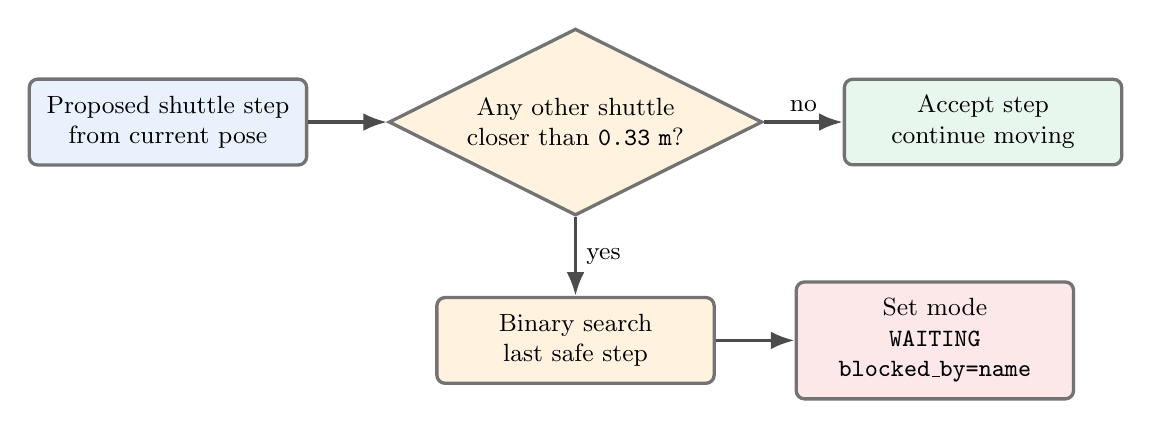
\begin{tikzpicture}[node distance=1.0cm and 1.0cm]
\node[flowbox, fill=flowblue] (proposal) {Proposed shuttle step\\from current pose};
\node[flowdecision, fill=floworange, right=of proposal] (distance) {Any other shuttle\\closer than \texttt{0.33 m}?};
\node[flowbox, fill=flowgreen, right=of distance] (move) {Accept step\\continue moving};
\node[flowbox, fill=floworange, below=of distance] (search) {Binary search\\last safe step};
\node[flowbox, fill=flowred, right=of search] (wait) {Set mode\\\texttt{WAITING}\\\texttt{blocked\_by=name}};

\draw[flowarrow] (proposal) -- (distance);
\draw[flowarrow] (distance) -- node[above, font=\small] {no} (move);
\draw[flowarrow] (distance) -- node[right, font=\small] {yes} (search);
\draw[flowarrow] (search) -- (wait);
\end{tikzpicture}}
\caption{Collision avoidance logic. The node does not use contact dynamics in
this phase; it prevents overlap by stopping at the last safe kinematic pose.}
\label{fig:collision-avoidance-flow}
\end{figure}

\chapter{Validation Procedures}

\section{CSV and graph validation}

\codenext{10}
\begin{lstlisting}[style=terminalcode,caption={Room 315 preprocessing and validation commands.}]
cd /home/tiago/ALI_ros2_ws
source /opt/ros/jazzy/setup.bash
source install/setup.bash

ros2 run mfja_robot_control_config room_315_csv_preprocessor.py
ros2 run mfja_robot_control_config room_315_network_validator.py
ros2 run mfja_robot_control_config room_315_continuous_path_validator.py
ros2 run mfja_robot_control_config room_315_segment_plot.py
\end{lstlisting}

The expected validation result is:

\begin{lstlisting}[style=terminalcode]
Status: PASS (0 warnings)
\end{lstlisting}

\begin{figure}[p]
\centering
\resizebox{0.95\textwidth}{!}{%
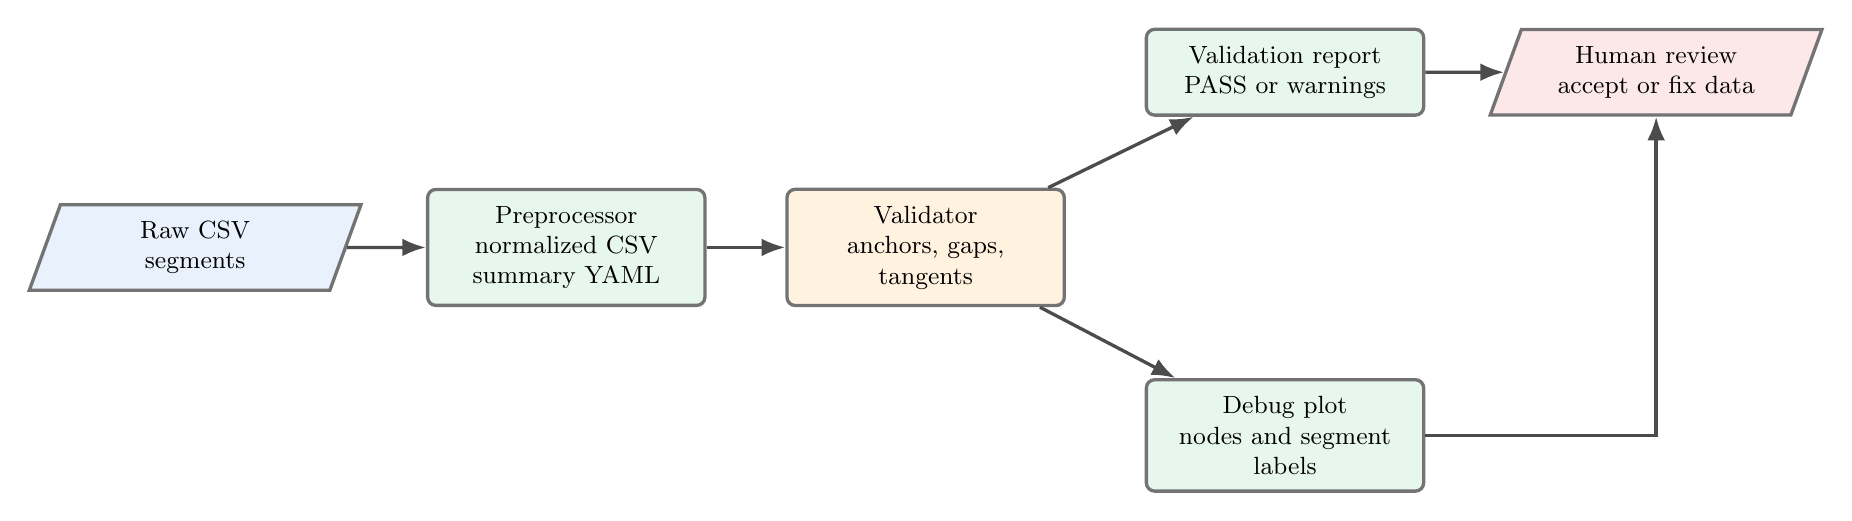
\begin{tikzpicture}[node distance=0.9cm and 1.0cm]
\node[flowio, fill=flowblue] (raw) {Raw CSV\\segments};
\node[flowbox, fill=flowgreen, right=of raw] (pre) {Preprocessor\\normalized CSV\\summary YAML};
\node[flowbox, fill=floworange, right=of pre] (val) {Validator\\anchors, gaps,\\tangents};
\node[flowbox, fill=flowgreen, above right=of val] (report) {Validation report\\PASS or warnings};
\node[flowbox, fill=flowgreen, below right=of val] (plot) {Debug plot\\nodes and segment\\labels};
\node[flowio, fill=flowred, right=of report] (review) {Human review\\accept or fix data};

\draw[flowarrow] (raw) -- (pre);
\draw[flowarrow] (pre) -- (val);
\draw[flowarrow] (val) -- (report);
\draw[flowarrow] (val) -- (plot);
\draw[flowarrow] (report) -- (review);
\draw[flowarrow] (plot) -| (review);
\end{tikzpicture}}
\caption{Validation workflow. The plots are not decorative; they are the visual
check that the CSV geometry, anchors, and directed graph agree with the physical
rail layout.}
\label{fig:validation-flow}
\end{figure}

\section{Runtime topics to inspect}

\codenext{10}
\begin{lstlisting}[style=terminalcode,caption={Runtime state and debug topics.}]
ros2 topic echo /room_315/shuttle/state --once
ros2 topic echo /room_315/sensors/switch_approach --once
ros2 topic echo /room_315/shuttle/pose_cmd --once
ros2 topic echo /room_315/shuttles/room315_shuttle_3/pose_cmd --once
ros2 topic echo /mfja/conveyor/switch_states --once
ros2 topic list | grep room_315
\end{lstlisting}

In the shuttle state output, the most important fields are:

\begin{itemize}
\item \texttt{entity\_name}: which shuttle the state describes;
\item \texttt{mode}: \texttt{MOVING}, \texttt{WAITING}, or \texttt{FALLING};
\item \texttt{enabled}: whether the shuttle is allowed to move;
\item \texttt{stopped\_by}: stopper name or \texttt{DISABLED};
\item \texttt{blocked\_by}: another shuttle that caused collision avoidance;
\item \texttt{switch\_states}: current route switch states;
\item \texttt{stopper\_states}: current stopper states.
\end{itemize}

\section{Expected negative tests}

\codenext{10}
\begin{lstlisting}[style=terminalcode,caption={Negative tests for start-slot rules.}]
# This should be rejected if slot 1 is still occupied.
ros2 topic pub --once /room_315/shuttle/add_cmd std_msgs/msg/String "{data: 'slot=1'}"

# This should always be rejected because only slots 1, 2, 3, and 4 are valid.
ros2 topic pub --once /room_315/shuttle/add_cmd std_msgs/msg/String "{data: 'slot=5'}"
\end{lstlisting}

The first command should produce an occupied-slot error when a shuttle is still
inside the start-slot occupancy radius. The second command should report that
the valid slots are \texttt{1}, \texttt{2}, \texttt{3}, and \texttt{4}.

\chapter{Current Operational Notes}

\begin{itemize}
\item Use \texttt{gazebo\_world\_name:=room\_315\_only} for the isolated Room
315 world.
\item Use \texttt{gazebo\_world\_name:=mfja\_3rd\_floor} for the full-floor
world.
\item If \texttt{Gazebo set\_pose service is not ready yet} appears, check the
world name and \texttt{ros2 service list}.
\item If a shuttle stops with \texttt{stopped\_by} set to a stopper name, open
that stopper through \texttt{/room\_315/stopper\_states}.
\item If a shuttle stops with \texttt{stopped\_by=DISABLED}, enable it again
through \texttt{/room\_315/shuttle/control\_cmd}.
\item If a shuttle enters \texttt{FALLING}, the graph has no valid successor for
the current switch configuration.
\item If a switch moves visually but routing does not change, send commands to
\texttt{/room\_315/switch\_states}, not directly to the visual switch topic.
\end{itemize}

\chapter{Detailed Implementation Walkthrough}

This chapter explains how the current implementation is organized internally.
It is written as a code-oriented engineering walkthrough, not only as an
operator guide. The goal is to make the current system understandable enough
that another developer can maintain it, extend it, or debug it during a live
demonstration.

\section{Design rule: topology is explicit, geometry is only geometry}

The most important design decision in Room 315 is that CSV geometry is not used
as the routing authority. CSV files describe points along each rail segment.
They are used to compute the shuttle pose and yaw at an arc-length position.
They are not used to guess which segment comes next by comparing endpoints.

The authoritative route logic lives in
\codepath{mfja_robot_control_config/config/room_315_kinematics/rail_network.yaml}.
That file declares the nodes, segment start and end nodes, switch rules,
fixed transitions, stopper locations, and start slots. This prevents fragile
behavior caused by tiny endpoint mismatches in the CSV files.

\section{How the rail paths were built from CSV files}

The Room 315 shuttle path was not drawn as one large loop in code. It was built
as a measured, directed rail network from CSV segment files. The CSV files are
the geometric input. The YAML network is the topological input. The Python core
combines both at runtime.

The complete path-building workflow is:

\begin{lstlisting}[style=terminalcode,caption={CSV-to-runtime workflow used for Room 315.}]
measured rail points
  -> CSV files with columns index,x,y,z
  -> one file per directed rail segment
  -> duplicate-point cleanup and normalization
  -> endpoint snapping to named anchors
  -> rail_network.yaml topology and routing
  -> validation report and debug plots
  -> arc-length geometry in the Python core
  -> ROS 2 node publishes Gazebo poses
\end{lstlisting}

\begin{figure}[p]
\centering
\resizebox{\textwidth}{!}{%
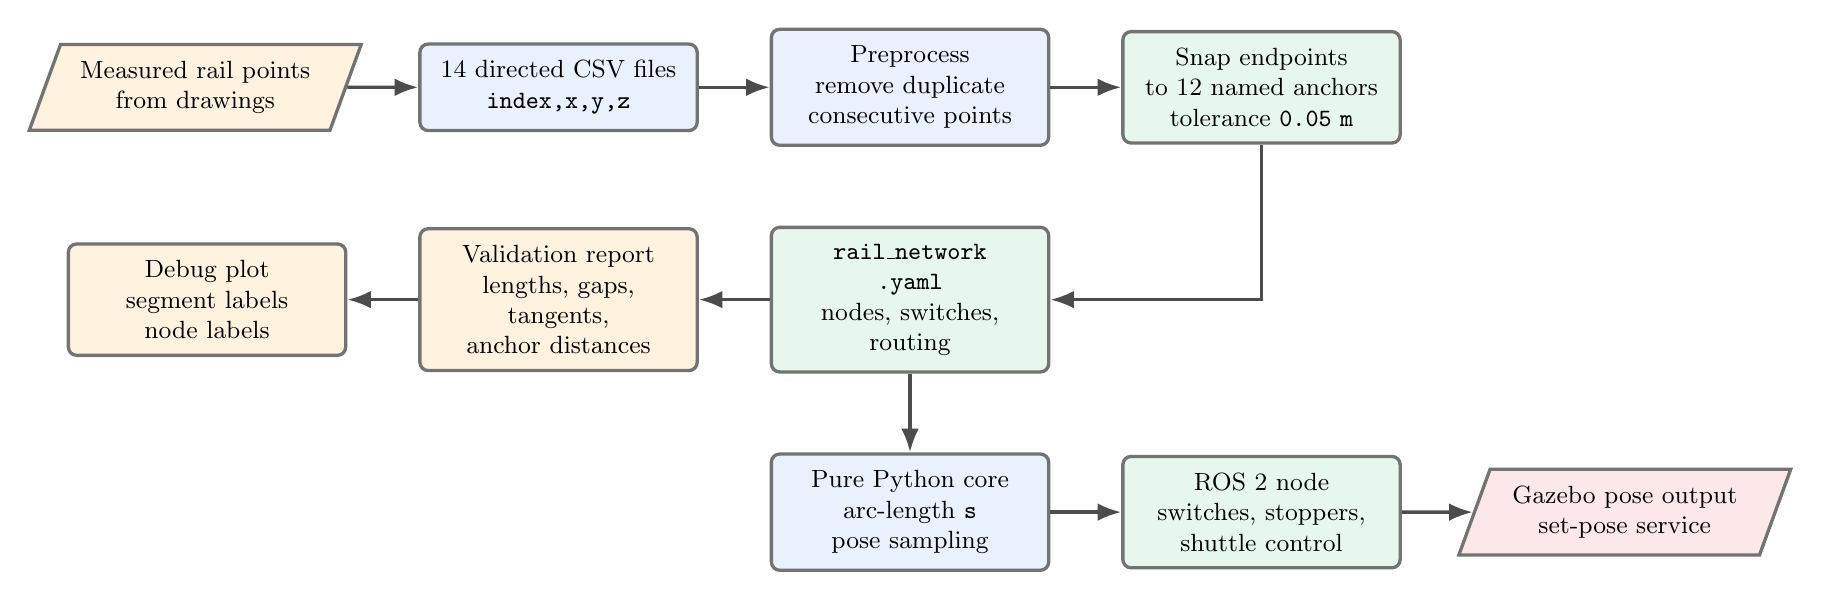
\begin{tikzpicture}[node distance=1.0cm and 0.9cm]
\node[flowio, fill=floworange] (measure) {Measured rail points\\from drawings};
\node[flowbox, fill=flowblue, right=of measure] (csv) {14 directed CSV files\\\texttt{index,x,y,z}};
\node[flowbox, fill=flowblue, right=of csv] (clean) {Preprocess\\remove duplicate\\consecutive points};
\node[flowbox, fill=flowgreen, right=of clean] (anchors) {Snap endpoints\\to 12 named anchors\\tolerance \texttt{0.05 m}};
\node[flowbox, fill=flowgreen, below=of clean] (yaml) {\texttt{rail\_network}\\\texttt{.yaml}\\nodes, switches, routing};
\node[flowbox, fill=floworange, left=of yaml] (validate) {Validation report\\lengths, gaps, tangents,\\anchor distances};
\node[flowbox, fill=floworange, left=of validate] (plot) {Debug plot\\segment labels\\node labels};
\node[flowbox, fill=flowblue, below=of yaml] (core) {Pure Python core\\arc-length \texttt{s}\\pose sampling};
\node[flowbox, fill=flowgreen, right=of core] (ros) {ROS 2 node\\switches, stoppers,\\shuttle control};
\node[flowio, fill=flowred, right=of ros] (gazebo) {Gazebo pose output\\set-pose service};

\draw[flowarrow] (measure) -- (csv);
\draw[flowarrow] (csv) -- (clean);
\draw[flowarrow] (clean) -- (anchors);
\draw[flowarrow] (anchors) |- (yaml);
\draw[flowarrow] (yaml) -- (validate);
\draw[flowarrow] (validate) -- (plot);
\draw[flowarrow] (yaml) -- (core);
\draw[flowarrow] (core) -- (ros);
\draw[flowarrow] (ros) -- (gazebo);
\end{tikzpicture}}
\caption{End-to-end flow chart for converting measured Room 315 rail data into
a running kinematic shuttle path. CSV files provide geometry. The YAML file
provides topology and routing. The ROS node combines both and publishes Gazebo
poses.}
\label{fig:csv-to-runtime-flow}
\end{figure}

\subsection*{Step 1: split the physical rail into directed segments}

The physical rail was split at the switch breakpoints. Each piece between two
important connection points became one segment. The current accepted segment
set is:

\begin{lstlisting}[style=terminalcode]
A1G A1S A2G A2S A3G A3S A4G A4S A12E A12I A14 A23 A34E A34I
\end{lstlisting}

Every segment has its own CSV file. Each CSV uses this schema:

\begin{lstlisting}[style=terminalcode]
index,x,y,z
0,-12.411...,...
1,-12.412...,...
...
\end{lstlisting}

The \texttt{index} column preserves the intended travel order. The shuttle
travels only from \texttt{index=0} toward the last row of that file. That rule
is important because the same physical rail shape could otherwise be interpreted
in two directions. The current network does not allow reverse traversal.

\subsection*{Step 2: keep CSV geometry separate from routing}

The CSV rows are used to compute where the shuttle is on a segment. They do not
decide which segment comes next. That decision comes only from
\texttt{rail\_network.yaml}. This separation prevents a common bug: two segment
endpoints can be physically connected but not numerically identical. If routing
used exact endpoint equality, tiny measurement or export errors could break the
graph.

The CSV geometry answers this question:

\begin{lstlisting}[style=terminalcode]
At distance s along segment A23, where is the shuttle pose?
\end{lstlisting}

The topology answers this question:

\begin{lstlisting}[style=terminalcode]
When A23 ends, which segment is valid under the current A3 switch state?
\end{lstlisting}

\subsection*{Step 3: preprocess and normalize the CSV files}

The preprocessing step reads the raw segment CSV files, removes duplicate
consecutive points, preserves the directed point order, and writes normalized
CSV files. Duplicate points are removed because a zero-length edge has no useful
direction and can create unstable yaw values.

The preprocessing command is:

\begin{lstlisting}[style=terminalcode]
ros2 run mfja_robot_control_config room_315_csv_preprocessor.py
\end{lstlisting}

The relevant inputs and outputs are:

\begin{itemize}
\item raw CSV input: \codepath{mfja_robot_control_config/config/room_315_kinematics/raw_segments};
\item normalized CSV output: \codepath{mfja_robot_control_config/config/room_315_kinematics/normalized_segments};
\item segment summary: \codepath{mfja_robot_control_config/config/room_315_kinematics/segment_summary.yaml}.
\end{itemize}

\subsection*{Step 4: create explicit node anchors}

After the geometry exists, endpoints are matched to named anchors. The current
network has twelve anchors:

\begin{lstlisting}[style=terminalcode]
A1_C A1_G A1_S
A2_C A2_G A2_S
A3_C A3_G A3_S
A4_C A4_G A4_S
\end{lstlisting}

The suffix meaning is:

\begin{itemize}
\item \texttt{C}: switch center or common connection point;
\item \texttt{G}: endpoint on the \texttt{G} branch;
\item \texttt{S}: endpoint on the \texttt{S} branch.
\end{itemize}

The validator snaps segment endpoints to these anchors using a tolerance of
\texttt{0.05 m}. Snapping here means validation association, not moving the
runtime shuttle by magic. The association says: this segment endpoint belongs to
this named node if it is close enough.

\subsection*{Step 5: define the graph and switch behavior}

After endpoints are attached to anchors, the YAML file defines how the directed
graph behaves. Fixed connections are simple. Switches are explicit. Converging
switches use guard logic so the shuttle fails if it approaches a branch that is
not selected.

The three rule types are:

\begin{itemize}
\item \texttt{fixed}: always move to the same next segment;
\item \texttt{switch\_select}: choose the outgoing branch from the switch state;
\item \texttt{switch\_guard}: allow entry only if the switch state matches the
incoming branch.
\end{itemize}

This is why the model is more precise than a simple "big loop/small loop"
toggle. The current state of each switch affects only the future route when the
shuttle reaches that switch. It does not teleport the shuttle or rewrite the
segment it is already on.

\subsection*{Step 6: validate visually and numerically}

The network validator checks the geometry and the topology together:

\begin{itemize}
\item segment lengths;
\item removed duplicate counts;
\item endpoint-to-anchor distances;
\item gaps above \texttt{0.05 m};
\item tangent mismatches above \texttt{25 deg};
\item whole-network debug plots with segment and node labels.
\end{itemize}

The validation command is:

\begin{lstlisting}[style=terminalcode]
ros2 run mfja_robot_control_config room_315_network_validator.py
\end{lstlisting}

The expected result for the current data is:

\begin{lstlisting}[style=terminalcode]
Status: PASS (0 warnings)
\end{lstlisting}

\begin{landscape}
\begin{figure}[p]
\centering
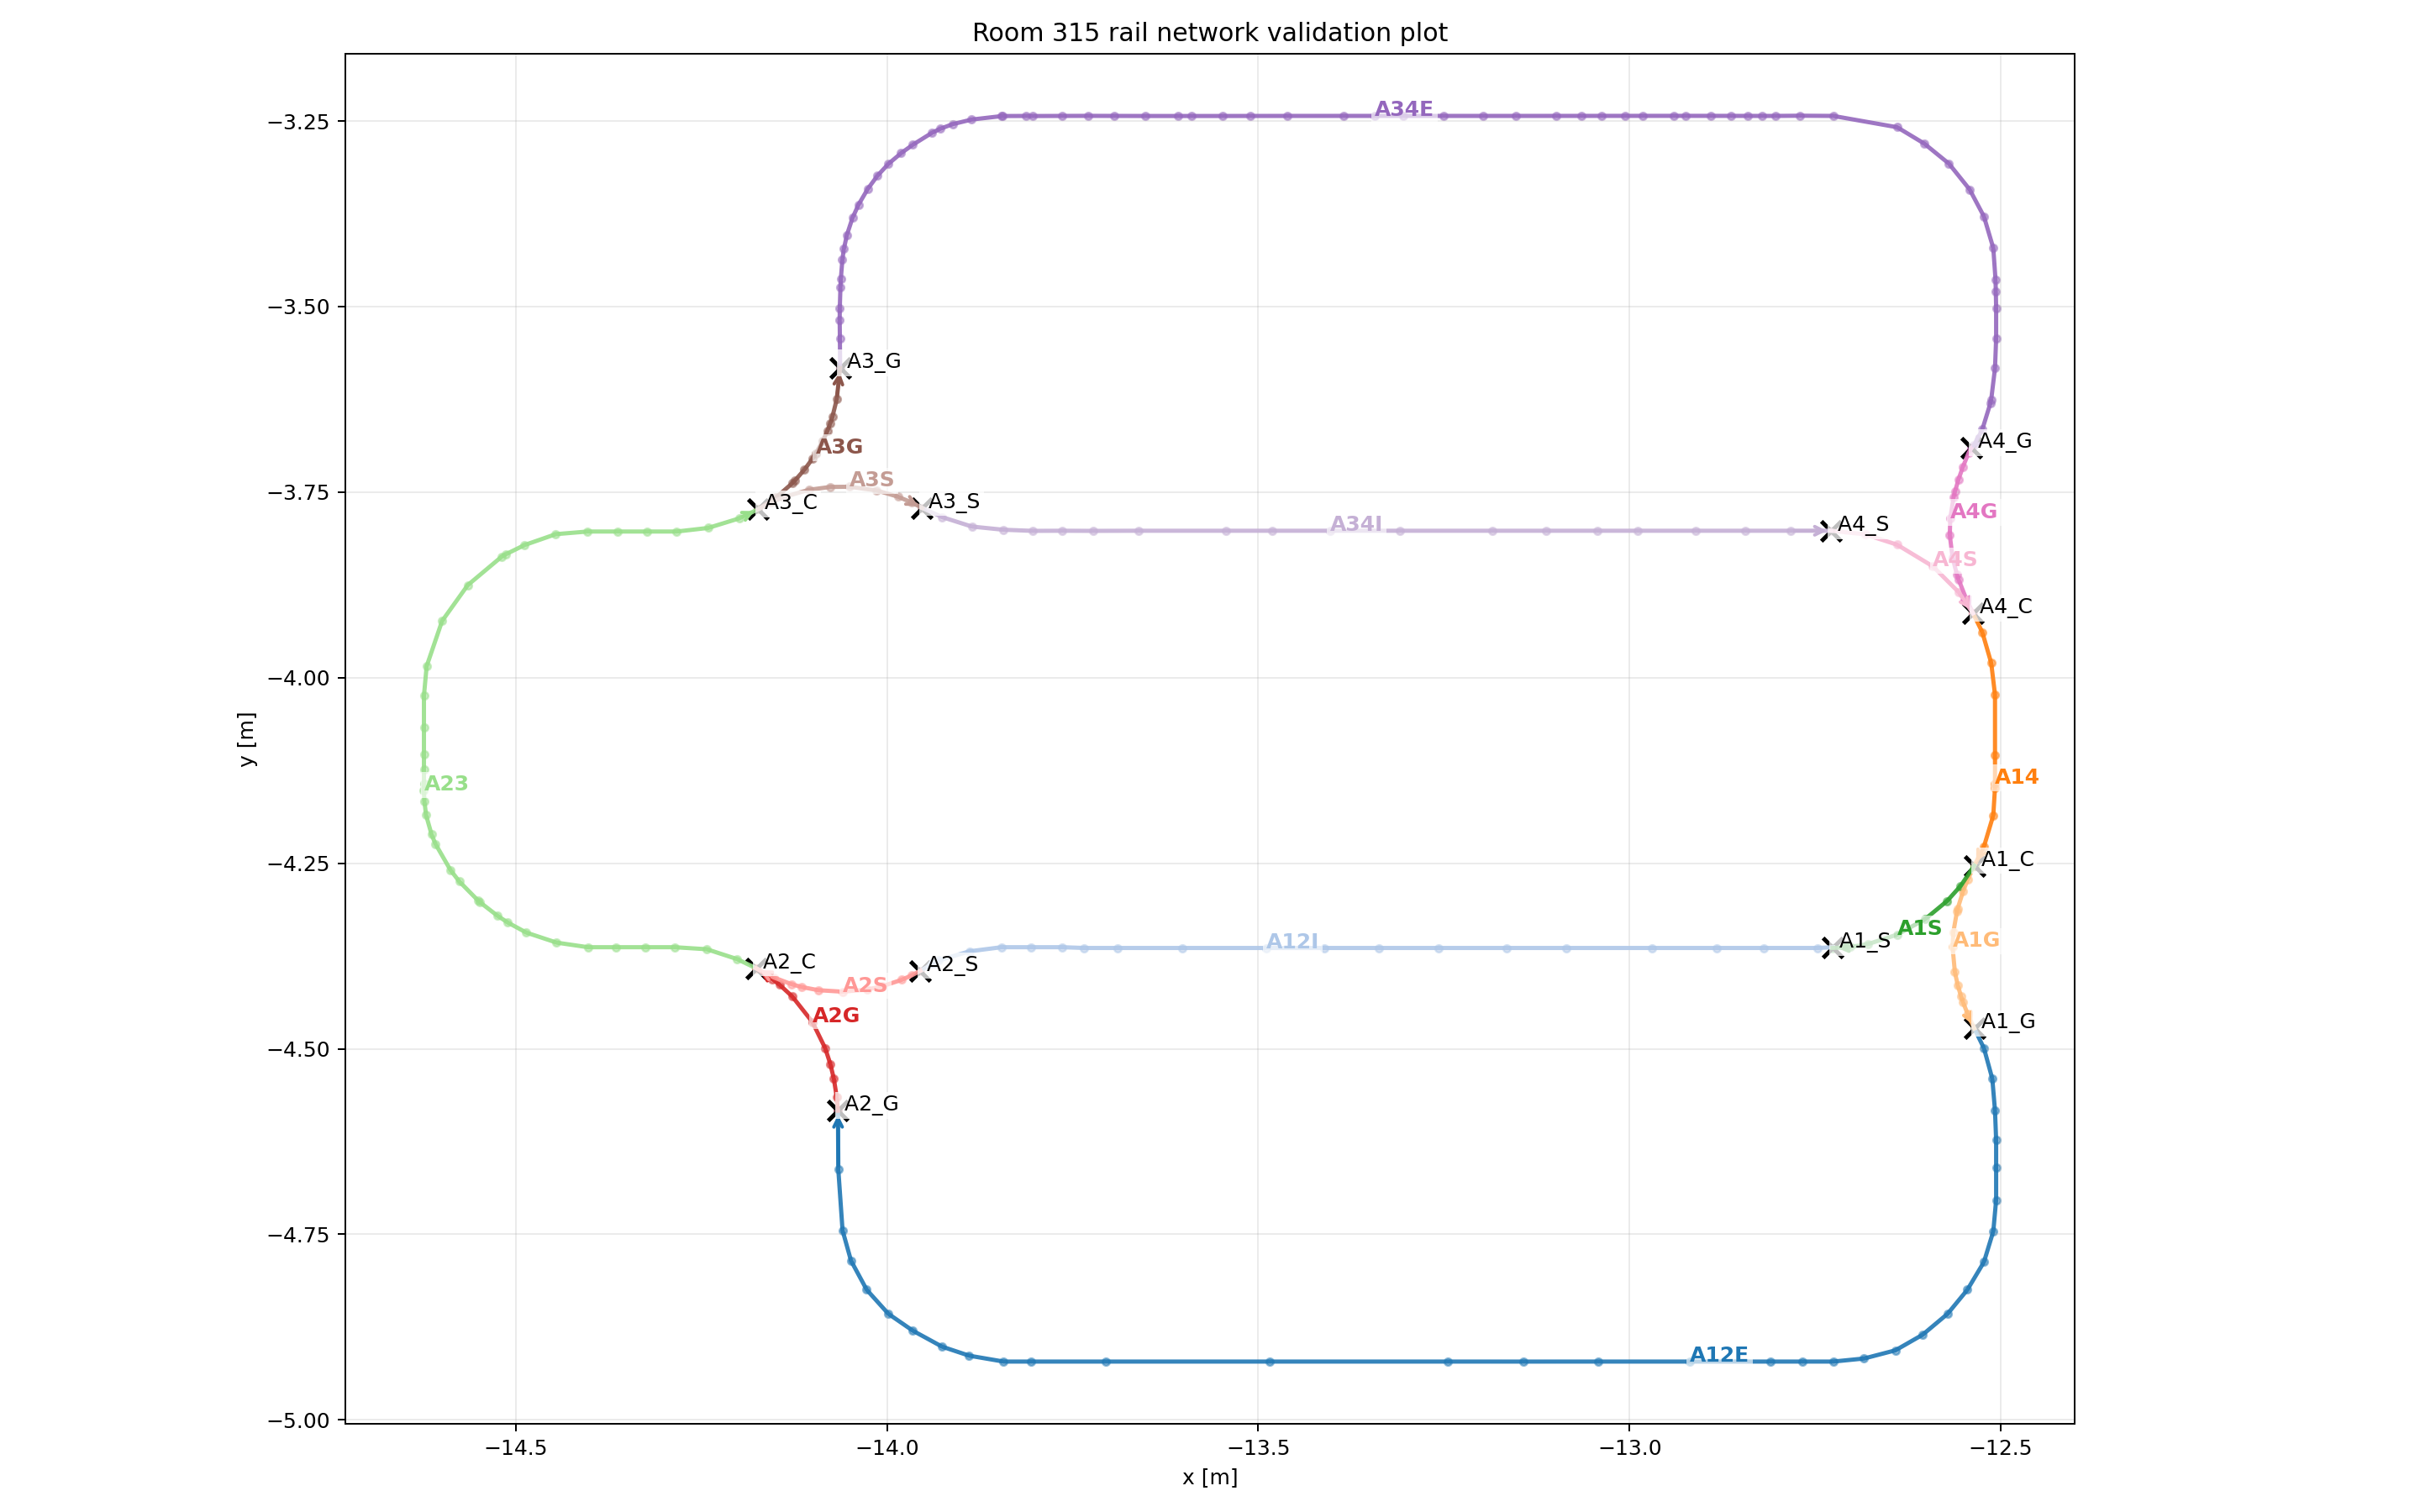
\includegraphics[width=0.90\linewidth]{mfja_robot_control_config/config/room_315_kinematics/debug_plots/network_validation.png}
\caption{Room 315 directed rail network validation plot. Segment labels show
the directed CSV segments. Node labels such as A1\_C, A1\_G, and A1\_S show the
explicit anchors used by the topology layer.}
\label{fig:room315-network-validation}
\end{figure}
\end{landscape}

\subsection*{Step 7: use arc length during simulation}

At runtime, the Python core converts each CSV polyline into cumulative
arc-length values. If the shuttle state says \texttt{current\_segment=A23} and
\texttt{s=0.40}, the core samples the point located \texttt{0.40 m} along
\texttt{A23}. Yaw is computed from the local CSV edge direction.

This gives the shuttle a continuous motion variable \texttt{s}, even though the
path is stored as discrete CSV rows. The shuttle never jumps from CSV point to
CSV point as a state machine. It interpolates along the polyline.

\begin{figure}[p]
\centering
\resizebox{0.92\textwidth}{!}{%
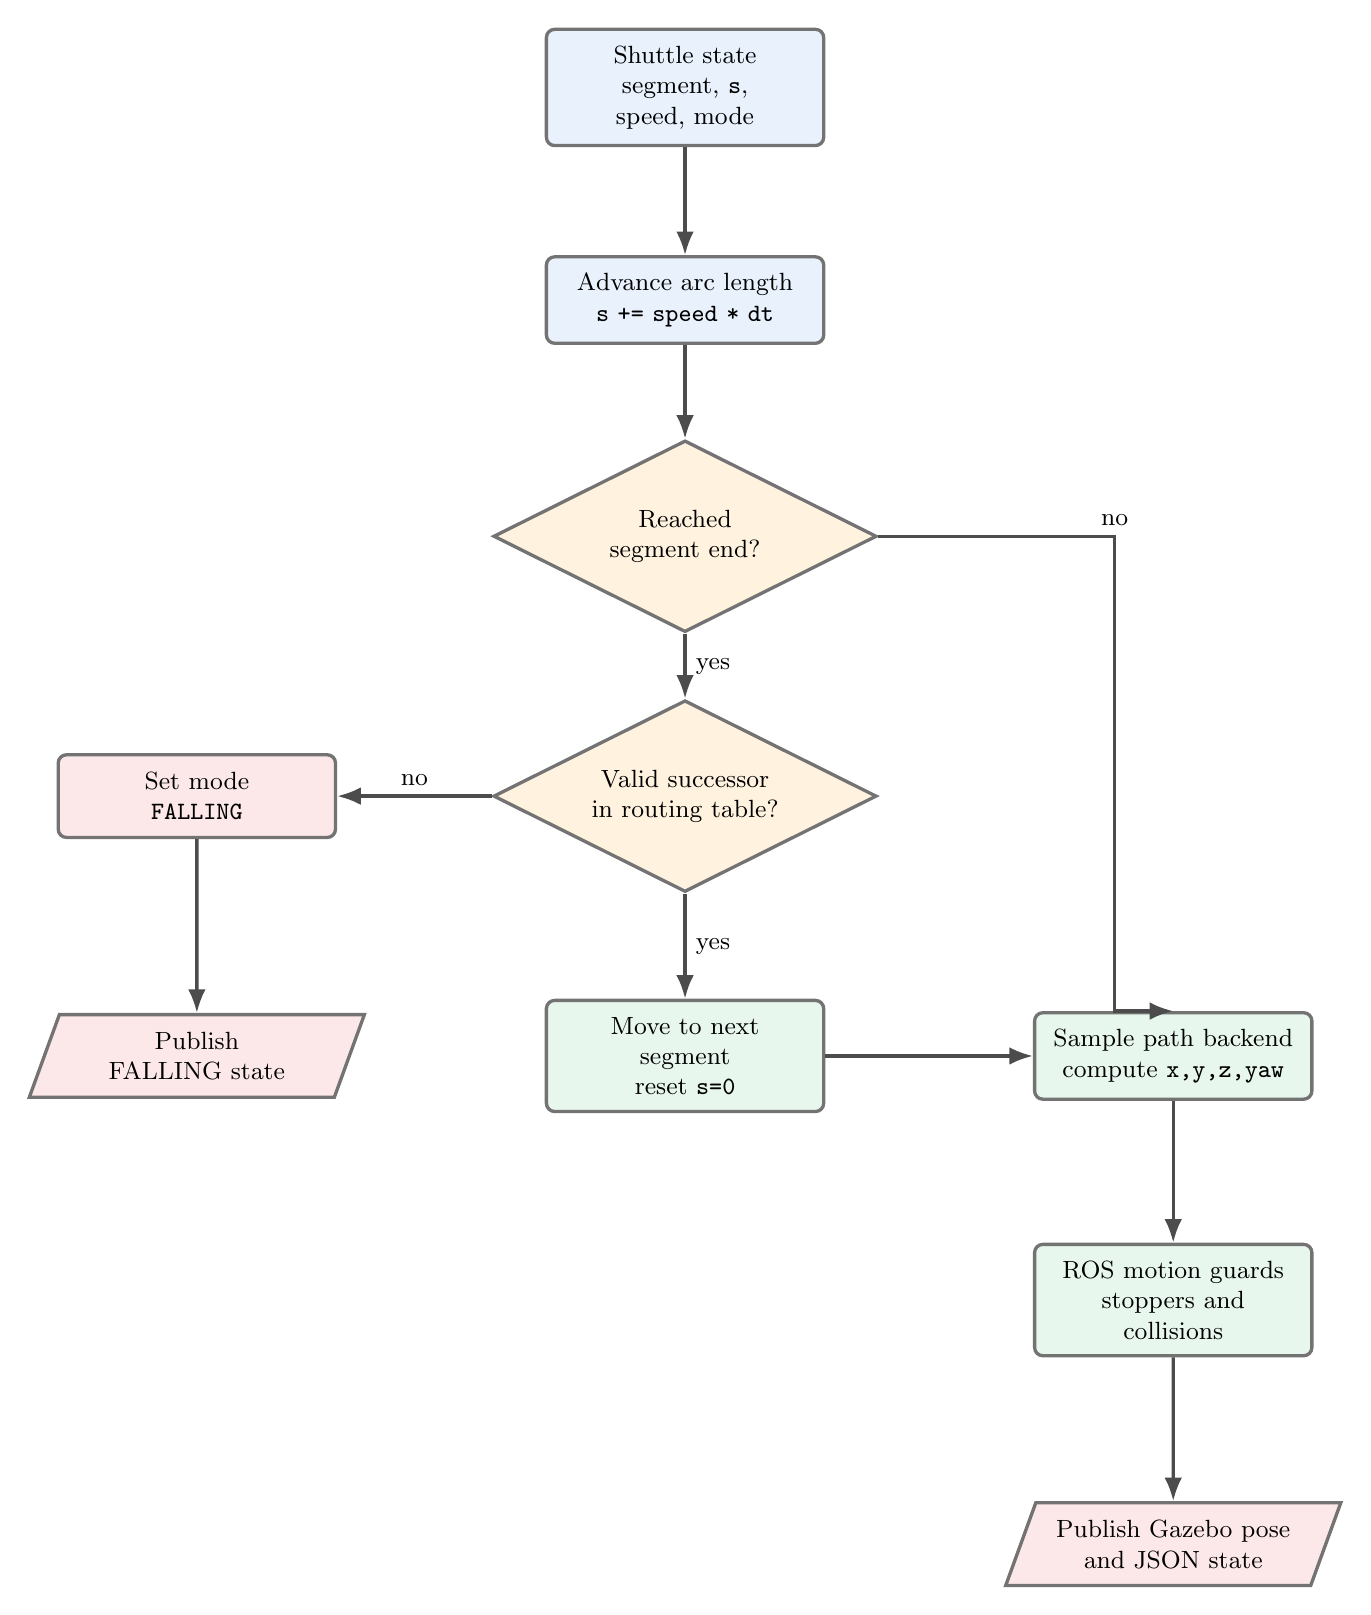
\begin{tikzpicture}[x=1cm,y=1cm]
\node[flowbox, fill=flowblue] (state) at (0,0) {Shuttle state\\segment, \texttt{s}, speed, mode};
\node[flowbox, fill=flowblue] (advance) at (0,-2.7) {Advance arc length\\\texttt{s += speed * dt}};
\node[flowdecision, fill=floworange] (end) at (0,-5.7) {Reached\\segment end?};
\node[flowdecision, fill=floworange] (route) at (0,-9.0) {Valid successor\\in routing table?};
\node[flowbox, fill=flowred] (falling) at (-6.2,-9.0) {Set mode\\\texttt{FALLING}};
\node[flowio, fill=flowred] (fallout) at (-6.2,-12.3) {Publish\\FALLING state};
\node[flowbox, fill=flowgreen] (next) at (0,-12.3) {Move to next segment\\reset \texttt{s=0}};
\node[flowbox, fill=flowgreen] (pose) at (6.2,-12.3) {Sample path backend\\compute \texttt{x,y,z,yaw}};
\node[flowbox, fill=flowgreen] (guards) at (6.2,-15.4) {ROS motion guards\\stoppers and collisions};
\node[flowio, fill=flowred] (output) at (6.2,-18.5) {Publish Gazebo pose\\and JSON state};

\draw[flowarrow] (state.south) -- (advance.north);
\draw[flowarrow] (advance.south) -- (end.north);
\draw[flowarrow] (end.south) -- node[right, font=\small] {yes} (route.north);
\draw[flowarrow] (end.east) -- ++(3.0,0) node[above, font=\small] {no} |- (pose.north);
\draw[flowarrow] (route.west) -- node[above, font=\small] {no} (falling.east);
\draw[flowarrow] (falling.south) -- (fallout.north);
\draw[flowarrow] (route.south) -- node[right, font=\small] {yes} (next.north);
\draw[flowarrow] (next.east) -- (pose.west);
\draw[flowarrow] (pose.south) -- (guards.north);
\draw[flowarrow] (guards.south) -- (output.north);
\end{tikzpicture}}
\caption{Runtime pose computation flow. The selected path backend is sampled by
arc length for geometry, while the routing table is consulted only when a
segment ends.}
\label{fig:runtime-pose-flow}
\end{figure}

\subsection*{Step 8: apply the route only at segment boundaries}

Switch states are checked when the shuttle reaches a segment end. Changing a
switch while the shuttle is in the middle of a segment changes only the future
successor. It does not move the shuttle to another branch immediately. This is
the behavior needed for a realistic kinematic-first model.

For example:

\begin{lstlisting}[style=terminalcode]
Shuttle is on A23.
A3 changes from G to S.
Shuttle stays on A23.
When A23 ends, the routing table selects A3S instead of A3G.
\end{lstlisting}

\subsection*{Step 9: bake accepted calibration into the CSV data}

During calibration, runtime scale and offset parameters were used to align the
shuttle path with the visible rail in Gazebo. Once the correct values were
found, the CSV coordinates were updated so normal operation no longer requires
manual scale and offset parameters. This makes startup simpler and less error
prone.

The normal node command should therefore use default pose scale and offset.
Runtime calibration parameters remain available only for future measurement
tests.

\codenext{22}
\lstinputlisting[
  style=reportcode,
  firstline=1,
  lastline=31,
  firstnumber=1,
  caption={Top-level Room 315 network policy and state spaces.}
]{mfja_robot_control_config/config/room_315_kinematics/rail_network.yaml}

The relevant behavior encoded here is:

\begin{itemize}
\item all rail segments are directed and forward-only;
\item a segment is traversed from CSV index \texttt{0} to the last CSV row;
\item reverse traversal is explicitly disabled;
\item if no valid successor exists, the shuttle enters \texttt{FALLING};
\item switch states are independent from stopper states;
\item topology and routing tables are the source of truth.
\end{itemize}

This is why the system does not silently auto-correct a bad path. If a switch
state makes the current rail branch invalid, the shuttle core reports a failure
state. That failure is useful during validation because it exposes topology
mistakes immediately instead of hiding them behind automatic rerouting.

\section{Start slots and physical entry poses}

The current system intentionally exposes only four valid start slots. These are
the four entry locations that were accepted for the current Room 315 phase.
The same values appear in both the YAML configuration and the Python fallback
constants. The YAML version is the preferred configuration source. The Python
constants keep the node usable if an older network file does not yet contain
\texttt{start\_slots}.

\codenext{28}
\lstinputlisting[
  style=reportcode,
  language=Python,
  firstline=80,
  lastline=130,
  firstnumber=80,
  caption={Start-slot fallback constants and per-shuttle runtime state.}
]{mfja_robot_control_config/scripts/room_315_kinematic_shuttle_node.py}

Each start slot contains a Gazebo pose in the order:

\begin{lstlisting}[style=terminalcode]
x y z roll pitch yaw
\end{lstlisting}

The current four slots are:

\begin{longtable}{@{}lllllll@{}}
\toprule
Slot & x & y & z & roll & pitch & yaw \\
\midrule
\endhead
\texttt{1} & \texttt{-14.95} & \texttt{-3.86} & \texttt{0.84} & \texttt{0.0} & \texttt{0.0} & \texttt{3.14} \\
\texttt{2} & \texttt{-15.43} & \texttt{-3.86} & \texttt{0.84} & \texttt{0.0} & \texttt{0.0} & \texttt{3.14} \\
\texttt{3} & \texttt{-15.24} & \texttt{-5.54} & \texttt{0.84} & \texttt{0.0} & \texttt{0.0} & \texttt{0.0} \\
\texttt{4} & \texttt{-14.77} & \texttt{-5.54} & \texttt{0.84} & \texttt{0.0} & \texttt{0.0} & \texttt{0.0} \\
\bottomrule
\end{longtable}

At startup, the node does not blindly put a shuttle on the pose and call it
valid. It snaps the requested start pose to the nearest point on the rail
network. The log message includes the selected segment, arc-length value, and
snap distance. A good startup line looks like this:

\begin{lstlisting}[style=terminalcode]
start_slot=2, start_segment=A34E, start_s=1.455, start_snap_distance=0.005 m
\end{lstlisting}

The snap distance is important. It tells the operator how far the configured
Gazebo start pose is from the rail geometry. A small value means the slot is
aligned with the rail. A large value means the configured slot should be
reviewed.

\section{ROS node parameter model}

The main runtime node is
\codepath{mfja_robot_control_config/scripts/room_315_kinematic_shuttle_node.py}.
It is intentionally parameter-driven so the same executable can be used in the
Room-only world and the full-floor world.

\codenext{40}
\lstinputlisting[
  style=reportcode,
  language=Python,
  firstline=137,
  lastline=190,
  firstnumber=137,
  caption={Main ROS node parameters for the kinematic shuttle system.}
]{mfja_robot_control_config/scripts/room_315_kinematic_shuttle_node.py}

The key parameter groups are:

\begin{itemize}
\item network and geometry parameters: \texttt{network\_yaml},
\texttt{path\_backend}, \texttt{arc\_length\_samples\_per\_edge}, and
\texttt{start\_snap\_tolerance\_m};
\item shuttle initialization: \texttt{shuttle\_count}, \texttt{start\_slot},
\texttt{start\_slots}, \texttt{gazebo\_entity\_name},
\texttt{gazebo\_entity\_names};
\item motion timing: \texttt{speed}, \texttt{update\_rate\_hz},
\texttt{gazebo\_set\_pose\_rate\_hz};
\item safety behavior: \texttt{enable\_collision\_avoidance},
\texttt{shuttle\_collision\_distance\_m},
\texttt{reject\_occupied\_start\_slots};
\item command topics: switch, stopper, shuttle add, shuttle ON/OFF, pose offset;
\item visual integration topics for the physical switch meshes;
\item Gazebo integration: world name, set-pose service, spawn service, and SDF
path;
\item pose transform and calibration parameters.
\end{itemize}

The default collision distance is \texttt{0.33 m}. It is enabled by default and
does not need to be written in normal terminal commands. This value was chosen
as the current practical stopping distance for the shuttle model in the
kinematic simulation.

\section{Loading start slots from the network file}

The node loads allowed start slots from
\texttt{rail\_network.yaml}. If the YAML file has no \texttt{start\_slots}
section, the code falls back to the Python constants shown earlier.

\codenext{20}
\lstinputlisting[
  style=reportcode,
  language=Python,
  firstline=421,
  lastline=438,
  firstnumber=421,
  caption={Allowed start-slot loading from \texttt{rail\_network.yaml}.}
]{mfja_robot_control_config/scripts/room_315_kinematic_shuttle_node.py}

This keeps configuration ownership clear: the network file owns the operational
start slots, and the node only provides defaults for compatibility.

\section{Stopper configuration and stop-point generation}

The stoppers are independent from switches. Each stopper is attached to the
approach side of a switch. A stopper does not decide the route. It only decides
whether an approaching shuttle must stop before the switch.

\codenext{36}
\lstinputlisting[
  style=reportcode,
  firstline=24,
  lastline=62,
  firstnumber=24,
  caption={Stopper definitions in the Room 315 network file.}
]{mfja_robot_control_config/config/room_315_kinematics/rail_network.yaml}

The YAML fields mean:

\begin{itemize}
\item \texttt{before\_switch}: the switch protected by this stopper;
\item \texttt{default\_state}: \texttt{0} means released, \texttt{1} means closed;
\item \texttt{stop\_offset\_m}: distance before the end of the approach segment;
\item \texttt{sensor\_distance\_m}: distance window where sensor events are
published;
\item \texttt{segments}: approach segments where the stopper can stop a shuttle.
\end{itemize}

The node converts each configured segment into a concrete stop point. If the
YAML does not specify an absolute arc-length \texttt{s}, the node computes:

\begin{lstlisting}[style=terminalcode]
stop_s = segment.length - stop_offset_m
\end{lstlisting}

\codenext{32}
\lstinputlisting[
  style=reportcode,
  language=Python,
  firstline=440,
  lastline=495,
  firstnumber=440,
  caption={Runtime loading of stopper definitions and stop-point conversion.}
]{mfja_robot_control_config/scripts/room_315_kinematic_shuttle_node.py}

This keeps the YAML readable while still giving the motion core a precise
arc-length stop location.

\section{Switches, fixed transitions, and routing table}

Switches are stored separately from fixed transitions. The switch section is
human-readable: it explains which node is controlled and which outgoing branch
belongs to each state.

\codenext{42}
\lstinputlisting[
  style=reportcode,
  firstline=296,
  lastline=357,
  firstnumber=296,
  caption={Switch declarations and fixed transitions.}
]{mfja_robot_control_config/config/room_315_kinematics/rail_network.yaml}

The runtime core does not infer route behavior from names. It reads the
\texttt{routing\_table}. The routing table is the executable graph policy.

\codenext{34}
\lstinputlisting[
  style=reportcode,
  firstline=358,
  lastline=390,
  firstnumber=358,
  caption={Routing table excerpt showing select, guard, and fixed rules.}
]{mfja_robot_control_config/config/room_315_kinematics/rail_network.yaml}

There are three important routing patterns:

\begin{itemize}
\item \texttt{fixed}: the segment always continues to one known successor;
\item \texttt{switch\_select}: the switch chooses the next branch;
\item \texttt{switch\_guard}: the shuttle may continue only if the switch state
matches the branch it is physically approaching.
\end{itemize}

The guard behavior matters at converging switches. For example, if a shuttle is
on \texttt{A12E}, it can enter \texttt{A2G} only when switch \texttt{A2} is in
state \texttt{G}. If \texttt{A2} is in state \texttt{S}, the routing table
returns \texttt{FALLING}. This represents an invalid physical configuration,
not an automatic detour.

\section{Pure Python kinematic core}

The pure core is in
\codepath{mfja_robot_control_config/scripts/room_315_kinematic_shuttle.py}.
It has no Gazebo dependency and no ROS dependency. This is deliberate: the
network and one-shuttle logic can be tested offline before integrating with
simulation services.

\codenext{28}
\lstinputlisting[
  style=reportcode,
  language=Python,
  firstline=14,
  lastline=45,
  firstnumber=14,
  caption={Core shuttle state and pose data structures.}
]{mfja_robot_control_config/scripts/room_315_kinematic_shuttle.py}

The shuttle state is intentionally small:

\begin{itemize}
\item \texttt{current\_segment}: the active rail segment;
\item \texttt{s}: progress along that segment in meters;
\item \texttt{speed}: scalar speed in meters per second;
\item \texttt{mode}: \texttt{MOVING}, \texttt{WAITING}, or \texttt{FALLING}.
\end{itemize}

The pose returned by the core includes the interpolated \texttt{x},
\texttt{y}, \texttt{z}, and yaw, plus the current segment and mode.

\section{Arc-length path backends}

CSV rows are still the measured input. They are not discarded. The important
change is that the runtime geometry layer now has two path backends behind the
same \texttt{SegmentGeometry.sample(s)} interface:

\begin{itemize}
\item \texttt{polyline}: direct piecewise-linear interpolation between CSV
points. This is the reference and debug backend because it follows the
measurement data exactly.
\item \texttt{cubic\_hermite}: continuous cubic Hermite interpolation with
arc-length reparameterization. This is the recommended runtime backend because
it gives smoother position and yaw along curves.
\end{itemize}

The runtime state is still parameterized by arc length \texttt{s}. During each
update, the core asks the selected backend for the pose at distance \texttt{s}.
This keeps the routing code independent from the geometric representation.

\codenext{42}
\lstinputlisting[
  style=reportcode,
  language=Python,
  firstline=48,
  lastline=132,
  firstnumber=48,
  caption={Segment geometry now supports polyline and continuous cubic Hermite backends.}
]{mfja_robot_control_config/scripts/room_315_kinematic_shuttle.py}

The accepted policy is:

\begin{lstlisting}[style=terminalcode]
Recommended runtime backend: cubic_hermite
Reference/debug backend:    polyline
\end{lstlisting}

Keeping both backends is intentional. The continuous backend is better for
normal operation, but the polyline backend remains the baseline for debugging.
If a future path appears misaligned, the operator can immediately compare
\texttt{cubic\_hermite} against \texttt{polyline} to determine whether the
problem comes from the fitted path layer or from the original CSV geometry.

The practical improvement already made was to use corrected CSV extraction and
then bake the calibration scale and offset into the CSV coordinates. That is
why normal node startup no longer needs \texttt{pose\_scale\_x},
\texttt{pose\_scale\_y}, \texttt{pose\_offset\_x}, or
\texttt{pose\_offset\_y} for the accepted path alignment.

\section{Continuous path validation}

The continuous backend is validated against the CSV polyline before it is used
for demos. The validation tool loads the same \texttt{rail\_network.yaml} twice:
once with \texttt{polyline} and once with \texttt{cubic\_hermite}. It then
samples the continuous curve and reports:

\begin{itemize}
\item polyline length and continuous length;
\item length difference in meters and percent;
\item maximum and mean deviation from the CSV polyline;
\item endpoint deltas;
\item maximum yaw step between sampled continuous points;
\item warnings if the continuous path deviates too far from the measured CSV.
\end{itemize}

\begin{lstlisting}[style=terminalcode]
ros2 run mfja_robot_control_config room_315_continuous_path_validator.py
\end{lstlisting}

The current accepted result is:

\begin{lstlisting}[style=terminalcode]
Validated continuous paths for 14 segments.
Status: PASS (0 warnings)
\end{lstlisting}

\begin{landscape}
\begin{figure}[p]
\centering
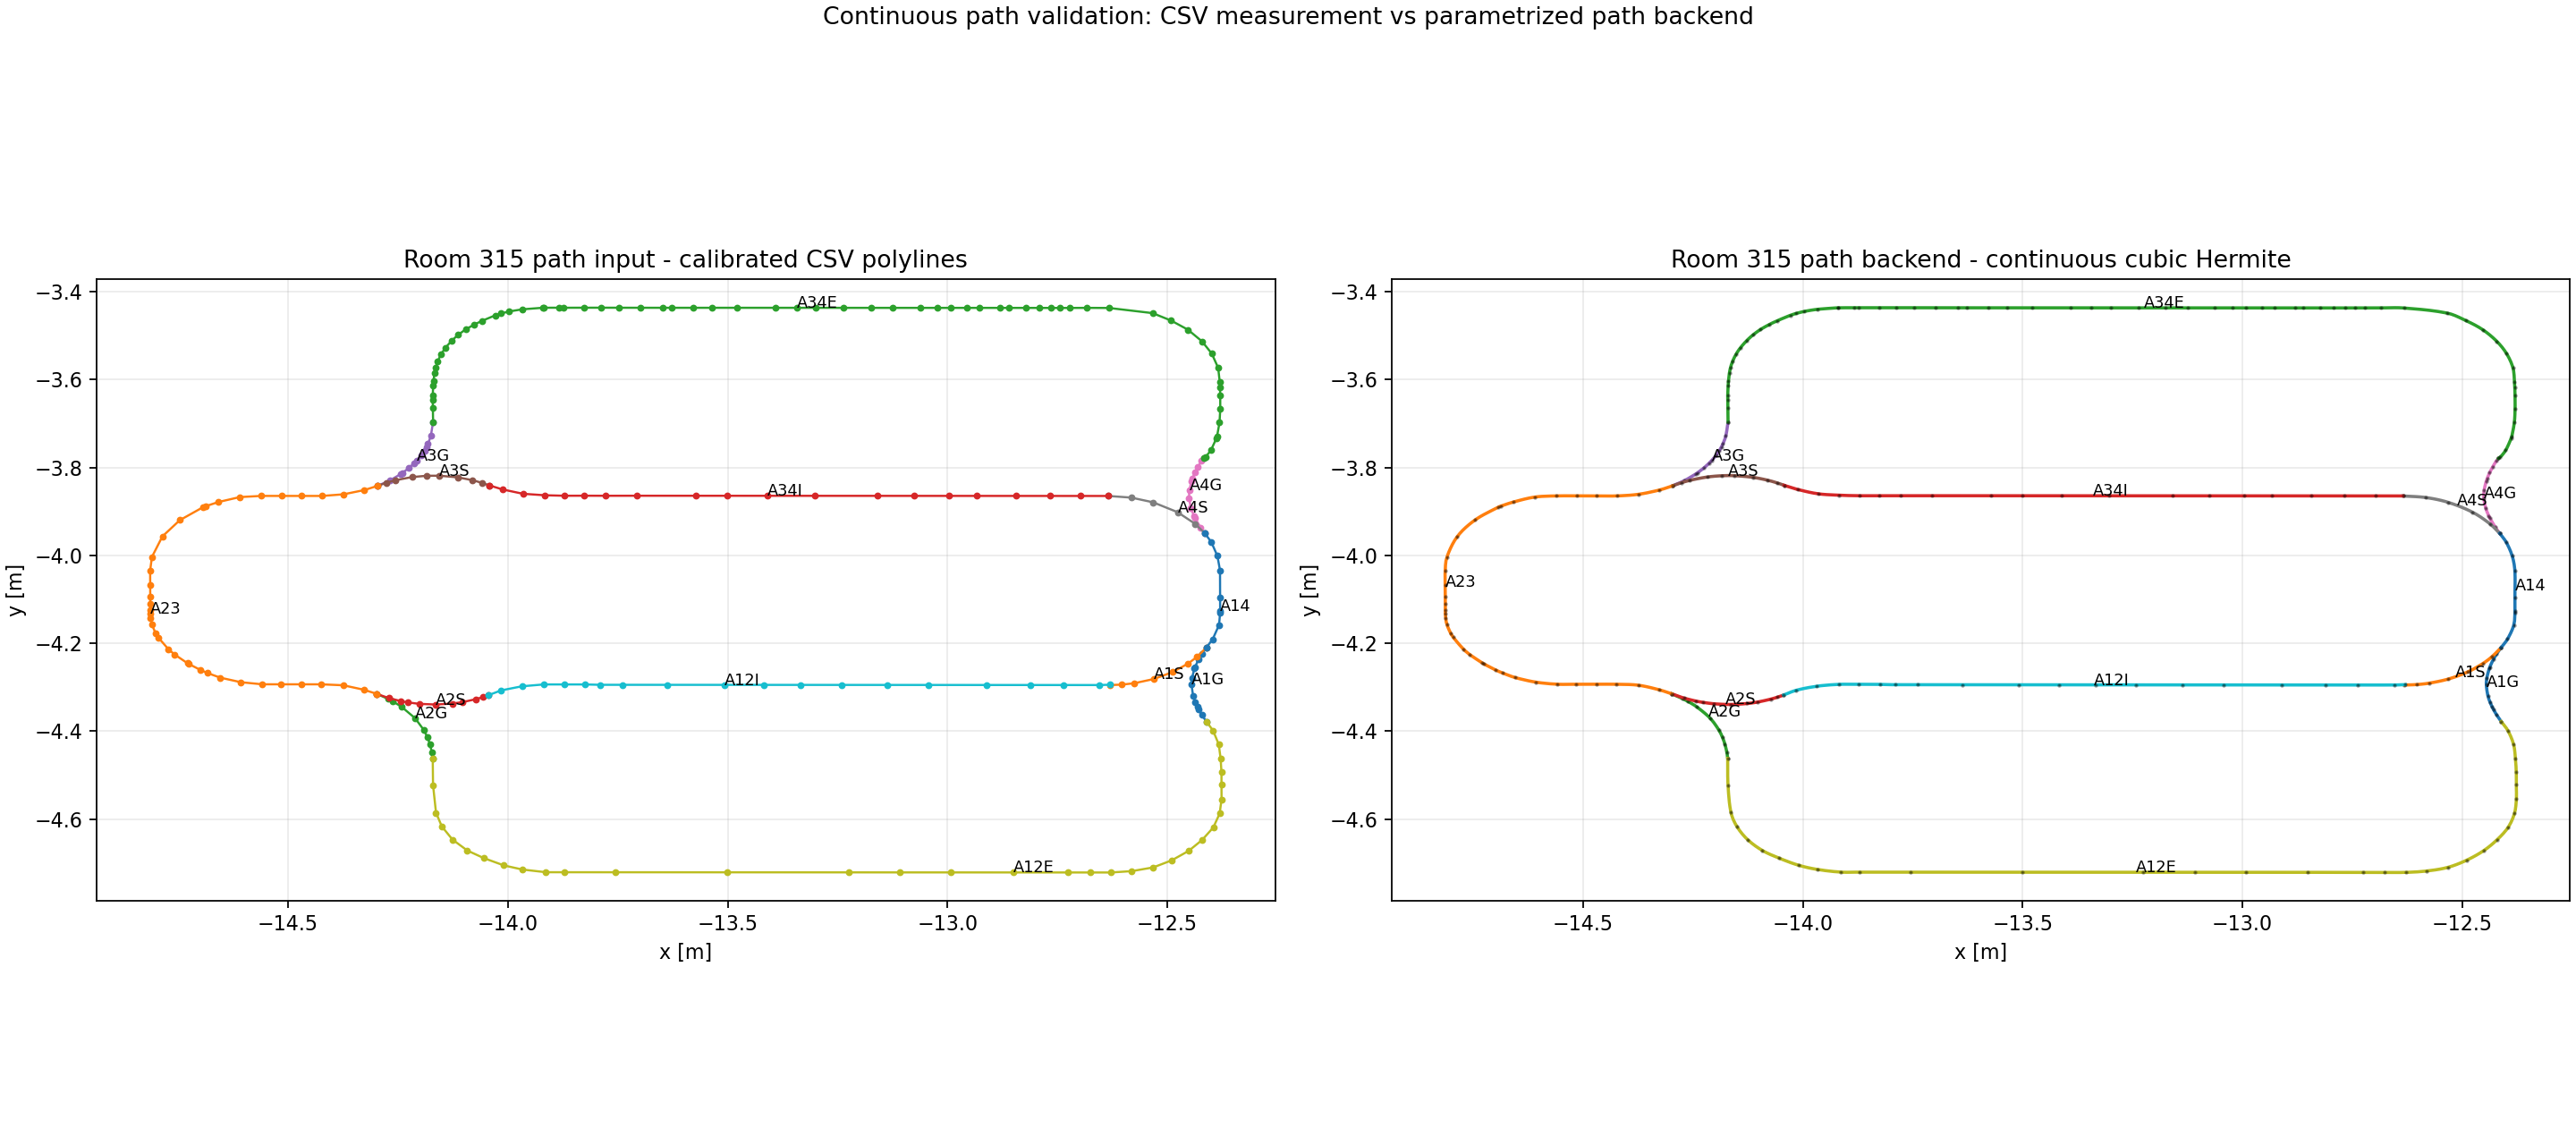
\includegraphics[width=0.94\linewidth]{mfja_robot_control_config/config/room_315_kinematics/debug_plots/continuous_path_validation.png}
\caption{Continuous path validation plot. The left side shows the calibrated
CSV polylines used as the reference measurement. The right side shows the
continuous cubic Hermite backend sampled densely. The black dots on the right
are the original CSV points, which makes it easy to detect overshoot.}
\label{fig:continuous-path-validation}
\end{figure}
\end{landscape}

\section{Successor resolution and explicit failure}

The core asks \texttt{RailNetwork.resolve\_successor()} what comes after the
current segment. If there is no successor, the shuttle enters
\texttt{FALLING}.

\codenext{42}
\lstinputlisting[
  style=reportcode,
  language=Python,
  firstline=95,
  lastline=156,
  firstnumber=95,
  caption={Rail network loading, switch normalization, and successor lookup.}
]{mfja_robot_control_config/scripts/room_315_kinematic_shuttle.py}

The function treats \texttt{FALLING} as a deliberate result. This is safer than
guessing a route because it tells the operator or developer that the current
switch configuration cannot support the current segment.

\section{Core stepping logic}

The step loop advances by \texttt{speed * dt}. If the remaining distance reaches
the end of the current segment, the core consumes that distance, resolves the
successor, and continues on the next segment. One update can cross more than one
short segment if the speed and time step allow it.

\codenext{34}
\lstinputlisting[
  style=reportcode,
  language=Python,
  firstline=179,
  lastline=214,
  firstnumber=179,
  caption={Pure kinematic stepping and FALLING behavior.}
]{mfja_robot_control_config/scripts/room_315_kinematic_shuttle.py}

The core does not know about stoppers, sensors, collision avoidance, Gazebo
spawning, or visual switch meshes. Those are ROS-node responsibilities layered
around the pure core.

\section{Runtime shuttle creation}

The node supports runtime shuttle addition through
\texttt{/room\_315/shuttle/add\_cmd}. The command parser accepts plain slot
numbers, assignment strings, and JSON payloads.

\codenext{44}
\lstinputlisting[
  style=reportcode,
  language=Python,
  firstline=627,
  lastline=706,
  firstnumber=627,
  caption={Runtime add-shuttle parser and occupied-slot rejection.}
]{mfja_robot_control_config/scripts/room_315_kinematic_shuttle_node.py}

The current default behavior is strict: if the requested start slot is occupied
inside the configured occupancy radius, the add request is rejected. This
matches the meeting requirement that adding a shuttle into an occupied start
location should say no instead of silently placing another shuttle there.

Examples of valid add commands are:

\begin{lstlisting}[style=terminalcode]
ros2 topic pub --once /room_315/shuttle/add_cmd std_msgs/msg/String "{data: 'slot=3'}"
ros2 topic pub --once /room_315/shuttle/add_cmd std_msgs/msg/String "{data: 'entity=room315_shuttle_5 slot=4 speed=0.2'}"
ros2 topic pub --once /room_315/shuttle/add_cmd std_msgs/msg/String "{data: '{\"slot\":\"2\",\"entity\":\"room315_shuttle_6\",\"speed\":\"0.15\"}'}"
\end{lstlisting}

Expected rejection examples are:

\begin{lstlisting}[style=terminalcode]
# Rejected if a shuttle is still inside the slot-1 occupancy radius.
ros2 topic pub --once /room_315/shuttle/add_cmd std_msgs/msg/String "{data: 'slot=1'}"

# Rejected because only slots 1, 2, 3, and 4 exist.
ros2 topic pub --once /room_315/shuttle/add_cmd std_msgs/msg/String "{data: 'slot=5'}"
\end{lstlisting}

\section{Stopper command implementation}

The stopper topic is
\texttt{/room\_315/stopper\_states}. The command is intentionally simple:
\texttt{0} means open or released, and \texttt{1} means closed or stop.

\codenext{22}
\lstinputlisting[
  style=reportcode,
  language=Python,
  firstline=995,
  lastline=1032,
  firstnumber=995,
  caption={Stopper command parser and accepted aliases.}
]{mfja_robot_control_config/scripts/room_315_kinematic_shuttle_node.py}

The accepted stopper aliases are useful during manual testing:

\begin{itemize}
\item closed state: \texttt{1}, \texttt{ON}, \texttt{STOP}, \texttt{CLOSED},
\texttt{BLOCK}, \texttt{TRUE};
\item open state: \texttt{0}, \texttt{OFF}, \texttt{OPEN}, \texttt{RELEASE},
\texttt{UNSTOP}, \texttt{FALSE};
\item selector: \texttt{A1}, \texttt{A2}, \texttt{A3}, \texttt{A4}, or
\texttt{ALL}.
\end{itemize}

Example commands:

\begin{lstlisting}[style=terminalcode]
ros2 topic pub --once /room_315/stopper_states std_msgs/msg/String "{data: 'A1=1'}"
ros2 topic pub --once /room_315/stopper_states std_msgs/msg/String "{data: 'A1=0'}"
ros2 topic pub --once /room_315/stopper_states std_msgs/msg/String "{data: 'A2=STOP A3=OPEN'}"
ros2 topic pub --once /room_315/stopper_states std_msgs/msg/String "{data: 'ALL=RELEASE'}"
\end{lstlisting}

\section{Per-shuttle ON/OFF implementation}

The shuttle ON/OFF topic is
\texttt{/room\_315/shuttle/control\_cmd}. It controls movement permission for
each shuttle independently. Turning a shuttle OFF does not delete it from
Gazebo. It leaves the shuttle controlled by the node, sets the mode to
\texttt{WAITING}, and marks \texttt{stopped\_by} as \texttt{DISABLED}.

\codenext{40}
\lstinputlisting[
  style=reportcode,
  language=Python,
  firstline=1034,
  lastline=1107,
  firstnumber=1034,
  caption={Per-shuttle ON/OFF control implementation.}
]{mfja_robot_control_config/scripts/room_315_kinematic_shuttle_node.py}

Accepted ON aliases include \texttt{1}, \texttt{ON}, \texttt{ENABLE},
\texttt{START}, \texttt{RUN}, and \texttt{TRUE}. Accepted OFF aliases include
\texttt{0}, \texttt{OFF}, \texttt{DISABLE}, \texttt{STOP}, \texttt{PAUSE}, and
\texttt{FALSE}.

Example commands:

\begin{lstlisting}[style=terminalcode]
ros2 topic pub --once /room_315/shuttle/control_cmd std_msgs/msg/String "{data: 'room315_shuttle_2=OFF'}"
ros2 topic pub --once /room_315/shuttle/control_cmd std_msgs/msg/String "{data: 'room315_shuttle_2=ON'}"
ros2 topic pub --once /room_315/shuttle/control_cmd std_msgs/msg/String "{data: 'ALL=OFF'}"
ros2 topic pub --once /room_315/shuttle/control_cmd std_msgs/msg/String "{data: 'ALL=ON'}"
ros2 topic pub --once /room_315/shuttle/control_cmd std_msgs/msg/String "{data: '{\"entity\":\"room315_shuttle_3\",\"enabled\":\"OFF\"}'}"
\end{lstlisting}

\section{Motion guard order}

The ROS node wraps the pure kinematic core with runtime motion guards. The
order is:

\begin{enumerate}
\item if the shuttle is disabled, keep it waiting;
\item if an active stopper is ahead, limit the step so the shuttle stops at the
stop point;
\item apply collision avoidance against already occupied shuttle poses;
\item if neither guard blocks the motion, let the pure kinematic core advance.
\end{enumerate}

\codenext{36}
\lstinputlisting[
  style=reportcode,
  language=Python,
  firstline=1382,
  lastline=1455,
  firstnumber=1382,
  caption={Motion guard wrapper for disabled shuttles and active stoppers.}
]{mfja_robot_control_config/scripts/room_315_kinematic_shuttle_node.py}

This order matters. A disabled shuttle should not move even if the path is
clear. A closed stopper should stop a shuttle before the switch. Collision
avoidance then prevents two active shuttles from merging into each other.

\section{Collision avoidance behavior}

Collision avoidance uses center-distance checks between the Gazebo-space poses
of shuttles. The default threshold is \texttt{0.33 m}. If the proposed full
time step would collide, the code performs a binary search over the time step
and moves only to the last safe position, then enters \texttt{WAITING}.

\codenext{34}
\lstinputlisting[
  style=reportcode,
  language=Python,
  firstline=1457,
  lastline=1517,
  firstnumber=1457,
  caption={Collision avoidance with binary search for the last safe step.}
]{mfja_robot_control_config/scripts/room_315_kinematic_shuttle_node.py}

This is a kinematic approximation, not full contact physics. It is intentionally
simple for the current phase. Its purpose is to prevent visual overlap and to
model the practical rule: if a shuttle reaches another shuttle, it waits instead
of passing through it.

\section{Sensor event publication}

The sensor interface is educational and workflow-oriented. It publishes
approach events whenever a shuttle is within the configured sensor distance
before a stopper.

\codenext{28}
\lstinputlisting[
  style=reportcode,
  language=Python,
  firstline=1648,
  lastline=1681,
  firstnumber=1648,
  caption={Switch-approach sensor event generation.}
]{mfja_robot_control_config/scripts/room_315_kinematic_shuttle_node.py}

A sensor event contains:

\begin{itemize}
\item \texttt{sensor}: for example \texttt{A3\_APPROACH};
\item \texttt{stopper}: the stopper that can stop the shuttle;
\item \texttt{before\_switch}: the protected switch;
\item \texttt{entity\_name}: which shuttle triggered the event;
\item \texttt{segment}: which segment the shuttle is currently on;
\item \texttt{distance\_m}: remaining distance to the stop point;
\item \texttt{stopper\_state}: whether the stopper is currently open or closed;
\item \texttt{workflow}: the intended sequence,
\texttt{sensor -> stop shuttle -> move switch -> unstop shuttle}.
\end{itemize}

When four shuttles are running, the sensor topic can contain events from any of
them. The event is not anonymous. The \texttt{entity\_name} field tells exactly
which shuttle the event belongs to.

\section{Published state payload}

The state topic is \texttt{/room\_315/shuttle/state}. It publishes a JSON string
with global switch and stopper states plus a list of shuttles. Each shuttle
entry includes the raw rail pose, transformed Gazebo pose, segment, arc length,
mode, enabled flag, blocker name, stopper name, start slot, and speed.

\codenext{28}
\lstinputlisting[
  style=reportcode,
  language=Python,
  firstline=1683,
  lastline=1705,
  firstnumber=1683,
  caption={Per-shuttle state fields published on the state topic.}
]{mfja_robot_control_config/scripts/room_315_kinematic_shuttle_node.py}

This topic is the best first debug topic because it tells whether a shuttle is
stopped by an OFF command, stopped by a stopper, blocked by another shuttle, or
in \texttt{FALLING}.

\chapter{Complete Feature Usage Manual}

This chapter lists the practical commands for every current feature. The
commands are intentionally copy-and-paste friendly.

\section{Terminal setup used by all examples}

Every terminal should start with:

\begin{lstlisting}[style=terminalcode]
cd /home/tiago/ALI_ros2_ws
source /opt/ros/jazzy/setup.bash
source install/setup.bash
\end{lstlisting}

If the workspace was modified, rebuild first:

\begin{lstlisting}[style=terminalcode]
cd /home/tiago/ALI_ros2_ws
source /opt/ros/jazzy/setup.bash

colcon build --base-paths \
  src/mfja_3rd_floor_gz/mfja_robot_control_config \
  src/mfja_3rd_floor_gz/mfja_3rd_floor_description \
  src/mfja_3rd_floor_gz/mfja_room_315_bringup \
  src/mfja_3rd_floor_gz/mfja_3rd_floor_bringup \
  src/mfja_3rd_floor_gz/mfja_3rd_floor_gz \
  --packages-select \
  mfja_robot_control_config \
  mfja_3rd_floor_description \
  mfja_room_315_bringup \
  mfja_3rd_floor_bringup \
  mfja_3rd_floor_gz \
  --symlink-install

source install/setup.bash
\end{lstlisting}

\section{Complete feature checklist}

The current repository contains both the older multi-robot simulation work and
the newer Room 315 kinematic shuttle work. The table below maps each feature to
the practical section that explains how to run it.

\begingroup
\small
\begin{longtable}{@{}p{0.28\textwidth}p{0.60\textwidth}@{}}
\toprule
Feature & Where it is operated from \\
\midrule
\endhead
Build and source the workspace & Terminal setup section in this chapter. \\
\addlinespace
Launch Room 315 only & \texttt{mfja\_room\_315\_bringup room\_315\_only.launch.py}. \\
\addlinespace
Launch the full third floor & \texttt{mfja\_3rd\_floor\_bringup full\_floor.launch.py}. \\
\addlinespace
Spawn no robots, selected robots, or all robots &
The \texttt{robots:=...} launch argument. \\
\addlinespace
Control industrial robot arms &
Namespaced \texttt{/robot\_name/joint\_trajectory} topics. \\
\addlinespace
Control the TIAGo mobile base &
The \texttt{/tiago1/cmd\_vel} topic. \\
\addlinespace
Run synchronized robot motions &
\texttt{multi\_robot\_sync\_demo.py}. \\
\addlinespace
Run one or more Room 315 shuttles &
\texttt{room\_315\_kinematic\_shuttle\_node.py}. \\
\addlinespace
Add shuttles during simulation &
\texttt{/room\_315/shuttle/add\_cmd}. \\
\addlinespace
Turn shuttles ON or OFF &
\texttt{/room\_315/shuttle/control\_cmd}. \\
\addlinespace
Change route switches &
\texttt{/room\_315/switch\_states}. \\
\addlinespace
Stop and release shuttles before switches &
\texttt{/room\_315/stopper\_states}. \\
\addlinespace
Read educational sensor events &
\texttt{/room\_315/sensors/switch\_approach}. \\
\addlinespace
Inspect shuttle state and collision holds &
\texttt{/room\_315/shuttle/state}. \\
\addlinespace
Validate CSV paths and the rail network &
\texttt{room\_315\_csv\_preprocessor.py},
\texttt{room\_315\_network\_validator.py}, and
\texttt{room\_315\_segment\_plot.py}. \\
\bottomrule
\end{longtable}
\endgroup

\section{Terminal 1: run Room 315 only}

Use this when testing Room 315 in isolation:

\begin{lstlisting}[style=terminalcode]
cd /home/tiago/ALI_ros2_ws
source /opt/ros/jazzy/setup.bash
source install/setup.bash

ros2 launch mfja_room_315_bringup room_315_only.launch.py \
  robots:=none \
  start_paused:=false
\end{lstlisting}

If Gazebo opens paused, press the play button or restart with
\texttt{start\_paused:=false}.

\section{Terminal 1 alternative: run the full floor}

Use this when testing Room 315 inside the complete third-floor world:

\begin{lstlisting}[style=terminalcode]
cd /home/tiago/ALI_ros2_ws
source /opt/ros/jazzy/setup.bash
source install/setup.bash

ros2 launch mfja_3rd_floor_bringup full_floor.launch.py \
  robots:=none \
  start_paused:=false
\end{lstlisting}

The shuttle node must use the same Gazebo world name as the running world. For
Room-only, use \texttt{room\_315\_only}. For the full floor, use
\texttt{mfja\_3rd\_floor}.

\section{Terminal 1 robot launch options}

The launch argument \texttt{robots:=...} controls which robot models are spawned
with the world. It supports:

\begin{itemize}
\item \texttt{robots:=none}: start the world without robots, useful for shuttle-only testing;
\item no \texttt{robots} argument or \texttt{robots:=}: use the YAML
\texttt{enabled} flags;
\item \texttt{robots:=all}: spawn every robot entry from the selected YAML file;
\item full names such as \texttt{kuka1} and \texttt{tiago1};
\item shortcuts such as \texttt{kuka}, \texttt{staubli}, \texttt{hc10},
\texttt{hc10dt}, and \texttt{tiago};
\item numeric indices by YAML order such as \texttt{1,2,5}.
\end{itemize}

Room 315 with all configured robot entries:

\begin{lstlisting}[style=terminalcode]
cd /home/tiago/ALI_ros2_ws
source /opt/ros/jazzy/setup.bash
source install/setup.bash

ros2 launch mfja_room_315_bringup room_315_only.launch.py \
  robots:=all \
  start_paused:=false
\end{lstlisting}

Room 315 with selected robots only:

\begin{lstlisting}[style=terminalcode]
cd /home/tiago/ALI_ros2_ws
source /opt/ros/jazzy/setup.bash
source install/setup.bash

ros2 launch mfja_room_315_bringup room_315_only.launch.py \
  robots:=kuka1,staubli1,yaskawa_hc10_1 \
  start_paused:=false
\end{lstlisting}

Full floor with all enabled robots from \texttt{robots.yaml}:

\begin{lstlisting}[style=terminalcode]
cd /home/tiago/ALI_ros2_ws
source /opt/ros/jazzy/setup.bash
source install/setup.bash

ros2 launch mfja_3rd_floor_bringup full_floor.launch.py \
  start_paused:=false
\end{lstlisting}

Full floor with all configured robots, even if a YAML entry is disabled:

\begin{lstlisting}[style=terminalcode]
cd /home/tiago/ALI_ros2_ws
source /opt/ros/jazzy/setup.bash
source install/setup.bash

ros2 launch mfja_3rd_floor_bringup full_floor.launch.py \
  robots:=all \
  start_paused:=false
\end{lstlisting}

Full floor with selected robots by shortcuts:

\begin{lstlisting}[style=terminalcode]
cd /home/tiago/ALI_ros2_ws
source /opt/ros/jazzy/setup.bash
source install/setup.bash

ros2 launch mfja_3rd_floor_bringup full_floor.launch.py \
  robots:=kuka,staubli,hc10,hc10dt,tiago \
  start_paused:=false
\end{lstlisting}

\section{Robot terminal A: verify robot topics}

Open a new terminal after the world is running:

\begin{lstlisting}[style=terminalcode]
cd /home/tiago/ALI_ros2_ws
source /opt/ros/jazzy/setup.bash
source install/setup.bash

ros2 topic list | grep -E '^/(kuka1|staubli1|yaskawa_hc10_1|yaskawa_hc10dt_1|tiago1)/'

ros2 topic info /kuka1/joint_trajectory
ros2 topic info /staubli1/joint_trajectory
ros2 topic info /yaskawa_hc10_1/joint_trajectory
ros2 topic info /yaskawa_hc10dt_1/joint_trajectory
ros2 topic info /tiago1/joint_trajectory
ros2 topic info /tiago1/cmd_vel
\end{lstlisting}

The joint trajectory topics are ROS-to-Gazebo command topics. The joint state,
odometry, and progress topics can be inspected while the robots move:

\begin{lstlisting}[style=terminalcode]
ros2 topic echo /kuka1/joint_states
ros2 topic echo /staubli1/joint_states
ros2 topic echo /yaskawa_hc10_1/joint_states
ros2 topic echo /yaskawa_hc10dt_1/joint_states
ros2 topic echo /tiago1/odom
\end{lstlisting}

\section{Robot terminal B: command individual robot arms}

KUKA KR6 R900 sixx:

\begin{lstlisting}[style=terminalcode]
cd /home/tiago/ALI_ros2_ws
source /opt/ros/jazzy/setup.bash
source install/setup.bash

ros2 topic pub --once /kuka1/joint_trajectory \
trajectory_msgs/msg/JointTrajectory \
"{joint_names: ['joint_a1','joint_a2','joint_a3','joint_a4','joint_a5','joint_a6'], points: [{positions: [0.6,-1.0,1.1,0.0,0.6,0.0], time_from_start: {sec: 3, nanosec: 0}}]}"
\end{lstlisting}

Staeubli TX2-60L:

\begin{lstlisting}[style=terminalcode]
cd /home/tiago/ALI_ros2_ws
source /opt/ros/jazzy/setup.bash
source install/setup.bash

ros2 topic pub --once /staubli1/joint_trajectory \
trajectory_msgs/msg/JointTrajectory \
"{joint_names: ['joint_1','joint_2','joint_3','joint_4','joint_5','joint_6'], points: [{positions: [0.1,0.4,-0.6,0.0,0.5,0.0], time_from_start: {sec: 3, nanosec: 0}}]}"
\end{lstlisting}

Yaskawa HC10:

\begin{lstlisting}[style=terminalcode]
cd /home/tiago/ALI_ros2_ws
source /opt/ros/jazzy/setup.bash
source install/setup.bash

ros2 topic pub --once /yaskawa_hc10_1/joint_trajectory \
trajectory_msgs/msg/JointTrajectory \
"{joint_names: ['joint_1_s','joint_2_l','joint_3_u','joint_4_r','joint_5_b','joint_6_t'], points: [{positions: [0.0,-0.6,0.8,0.0,0.5,0.0], time_from_start: {sec: 3, nanosec: 0}}]}"
\end{lstlisting}

Yaskawa HC10DT:

\begin{lstlisting}[style=terminalcode]
cd /home/tiago/ALI_ros2_ws
source /opt/ros/jazzy/setup.bash
source install/setup.bash

ros2 topic pub --once /yaskawa_hc10dt_1/joint_trajectory \
trajectory_msgs/msg/JointTrajectory \
"{joint_names: ['joint_1_s','joint_2_l','joint_3_u','joint_4_r','joint_5_b','joint_6_t'], points: [{positions: [0.0,-0.5,0.7,0.0,0.4,0.0], time_from_start: {sec: 3, nanosec: 0}}]}"
\end{lstlisting}

TIAGo arm and head:

\begin{lstlisting}[style=terminalcode]
cd /home/tiago/ALI_ros2_ws
source /opt/ros/jazzy/setup.bash
source install/setup.bash

ros2 topic pub --once /tiago1/joint_trajectory \
trajectory_msgs/msg/JointTrajectory \
"{joint_names: ['torso_lift_joint','arm_1_joint','arm_2_joint','arm_3_joint','arm_4_joint','arm_5_joint','arm_6_joint','arm_7_joint','head_1_joint','head_2_joint'], points: [{positions: [0.10,0.3,-0.5,-0.4,1.0,0.2,-0.2,0.1,0.2,-0.2], time_from_start: {sec: 4, nanosec: 0}}]}"
\end{lstlisting}

\section{Robot terminal C: command the TIAGo base}

Move the TIAGo base slowly:

\begin{lstlisting}[style=terminalcode]
cd /home/tiago/ALI_ros2_ws
source /opt/ros/jazzy/setup.bash
source install/setup.bash

ros2 topic pub -r 20 /tiago1/cmd_vel geometry_msgs/msg/Twist \
"{linear: {x: 0.15, y: 0.0, z: 0.0}, angular: {x: 0.0, y: 0.0, z: 0.20}}"
\end{lstlisting}

Stop the TIAGo base from another terminal, or press Ctrl-C in the publishing
terminal and send one zero command:

\begin{lstlisting}[style=terminalcode]
cd /home/tiago/ALI_ros2_ws
source /opt/ros/jazzy/setup.bash
source install/setup.bash

ros2 topic pub --once /tiago1/cmd_vel geometry_msgs/msg/Twist \
"{linear: {x: 0.0, y: 0.0, z: 0.0}, angular: {x: 0.0, y: 0.0, z: 0.0}}"
\end{lstlisting}

\section{Robot terminal D: synchronized multi-robot commands}

List supported joints and default poses:

\begin{lstlisting}[style=terminalcode]
cd /home/tiago/ALI_ros2_ws
source /opt/ros/jazzy/setup.bash
source install/setup.bash

ros2 run mfja_robot_control_config multi_robot_sync_demo.py --list-joints
\end{lstlisting}

Move every enabled robot to its default preset:

\begin{lstlisting}[style=terminalcode]
cd /home/tiago/ALI_ros2_ws
source /opt/ros/jazzy/setup.bash
source install/setup.bash

ros2 run mfja_robot_control_config multi_robot_sync_demo.py \
  --trajectory-duration 4.0
\end{lstlisting}

Move only selected robots with explicit goals:

\begin{lstlisting}[style=terminalcode]
cd /home/tiago/ALI_ros2_ws
source /opt/ros/jazzy/setup.bash
source install/setup.bash

ros2 run mfja_robot_control_config multi_robot_sync_demo.py \
  --goal kuka1=1.2,-1.2,1.4,0.0,0.3,0.0 \
  --goal staubli1=0.1,0.4,-0.6,0.0,0.5,0.0 \
  --trajectory-duration 4.0
\end{lstlisting}

Move TIAGo arm and base together for a short demo:

\begin{lstlisting}[style=terminalcode]
cd /home/tiago/ALI_ros2_ws
source /opt/ros/jazzy/setup.bash
source install/setup.bash

ros2 run mfja_robot_control_config multi_robot_sync_demo.py \
  --goal tiago1=0.10,0.3,-0.5,-0.4,1.0,0.2,-0.2,0.1,0.2,-0.2 \
  --tiago-base-linear 0.10 \
  --tiago-base-angular 0.15 \
  --tiago-base-duration 3.0 \
  --trajectory-duration 4.0
\end{lstlisting}

\section{Terminal 2: bridge the Gazebo set-pose service}

For Room-only:

\begin{lstlisting}[style=terminalcode]
cd /home/tiago/ALI_ros2_ws
source /opt/ros/jazzy/setup.bash
source install/setup.bash
export GZ_PARTITION=room315

ros2 run ros_gz_bridge parameter_bridge \
  /world/room_315_only/set_pose@ros_gz_interfaces/srv/SetEntityPose
\end{lstlisting}

For the full floor:

\begin{lstlisting}[style=terminalcode]
cd /home/tiago/ALI_ros2_ws
source /opt/ros/jazzy/setup.bash
source install/setup.bash

ros2 run ros_gz_bridge parameter_bridge \
  /world/mfja_3rd_floor/set_pose@ros_gz_interfaces/srv/SetEntityPose
\end{lstlisting}

Check that the service exists:

\begin{lstlisting}[style=terminalcode]
ros2 service list | grep set_pose
\end{lstlisting}

\section{Terminal 3: run one shuttle}

Room-only one-shuttle command:

\begin{lstlisting}[style=terminalcode]
cd /home/tiago/ALI_ros2_ws
source /opt/ros/jazzy/setup.bash
source install/setup.bash

ros2 run mfja_robot_control_config room_315_kinematic_shuttle_node.py --ros-args \
  -p gazebo_world_name:=room_315_only \
  -p start_slot:=2 \
  -p enable_gazebo_set_pose:=true \
  -p gazebo_entity_name:=room315_shuttle_1 \
  -p speed:=0.2 \
  -p gazebo_set_pose_rate_hz:=10.0
\end{lstlisting}

Full-floor one-shuttle command:

\begin{lstlisting}[style=terminalcode]
cd /home/tiago/ALI_ros2_ws
source /opt/ros/jazzy/setup.bash
source install/setup.bash

ros2 run mfja_robot_control_config room_315_kinematic_shuttle_node.py --ros-args \
  -p gazebo_world_name:=mfja_3rd_floor \
  -p start_slot:=2 \
  -p enable_gazebo_set_pose:=true \
  -p gazebo_entity_name:=room315_shuttle_1 \
  -p speed:=0.2 \
  -p gazebo_set_pose_rate_hz:=10.0
\end{lstlisting}

\section{Terminal 3: four-shuttle startup}

\begin{lstlisting}[style=terminalcode]
cd /home/tiago/ALI_ros2_ws
source /opt/ros/jazzy/setup.bash
source install/setup.bash

ros2 run mfja_robot_control_config room_315_kinematic_shuttle_node.py --ros-args \
  -p gazebo_world_name:=room_315_only \
  -p shuttle_count:=4 \
  -p start_slots:=1,2,3,4 \
  -p gazebo_entity_names:=room315_shuttle_1,room315_shuttle_2,room315_shuttle_3,room315_shuttle_4 \
  -p enable_gazebo_set_pose:=true \
  -p speed:=0.2 \
  -p gazebo_set_pose_rate_hz:=10.0
\end{lstlisting}

If running in the full-floor world, change only:

\begin{lstlisting}[style=terminalcode]
-p gazebo_world_name:=mfja_3rd_floor
\end{lstlisting}

\section{Terminal 4: inspect state continuously}

\begin{lstlisting}[style=terminalcode]
cd /home/tiago/ALI_ros2_ws
source /opt/ros/jazzy/setup.bash
source install/setup.bash

ros2 topic echo /room_315/shuttle/state
\end{lstlisting}

Useful fields:

\begin{itemize}
\item \texttt{entity\_name}: identifies which shuttle the row belongs to;
\item \texttt{current\_segment}: current rail segment;
\item \texttt{s}: arc-length progress on that segment;
\item \texttt{mode}: \texttt{MOVING}, \texttt{WAITING}, or \texttt{FALLING};
\item \texttt{enabled}: per-shuttle ON/OFF state;
\item \texttt{stopped\_by}: stopper name or \texttt{DISABLED};
\item \texttt{blocked\_by}: another shuttle if collision avoidance is holding it;
\item \texttt{start\_slot}: original start slot used for that shuttle.
\end{itemize}

\section{Terminal 5: inspect sensor events}

\begin{lstlisting}[style=terminalcode]
cd /home/tiago/ALI_ros2_ws
source /opt/ros/jazzy/setup.bash
source install/setup.bash

ros2 topic echo /room_315/sensors/switch_approach
\end{lstlisting}

Example event:

\begin{lstlisting}[style=terminalcode]
data: '{"sensors": [{"before_switch": "A3", "distance_m": 0.214, "entity_name": "room315_shuttle_4", "segment": "A23", "sensor": "A3_APPROACH", "stopper": "A3", "stopper_state": "0", "workflow": "sensor -> stop shuttle -> move switch -> unstop shuttle"}], "stopper_states": {"A1": "0", "A2": "0", "A3": "0", "A4": "0"}}'
\end{lstlisting}

This means shuttle \texttt{room315\_shuttle\_4} is approaching switch
\texttt{A3} on segment \texttt{A23}. The remaining distance to the A3 stop
point is about \texttt{0.214 m}. The stopper is currently open because
\texttt{stopper\_state} is \texttt{0}.

\section{Switch commands}

Switches are controlled through:

\begin{lstlisting}[style=terminalcode]
/room_315/switch_states
\end{lstlisting}

Use these commands to test all switches:

\begin{lstlisting}[style=terminalcode]
ros2 topic pub --once /room_315/switch_states std_msgs/msg/String "{data: 'A1=G'}"
ros2 topic pub --once /room_315/switch_states std_msgs/msg/String "{data: 'A1=S'}"
ros2 topic pub --once /room_315/switch_states std_msgs/msg/String "{data: 'A2=G'}"
ros2 topic pub --once /room_315/switch_states std_msgs/msg/String "{data: 'A2=S'}"
ros2 topic pub --once /room_315/switch_states std_msgs/msg/String "{data: 'A3=G'}"
ros2 topic pub --once /room_315/switch_states std_msgs/msg/String "{data: 'A3=S'}"
ros2 topic pub --once /room_315/switch_states std_msgs/msg/String "{data: 'A4=G'}"
ros2 topic pub --once /room_315/switch_states std_msgs/msg/String "{data: 'A4=S'}"
\end{lstlisting}

Set all switches at once:

\begin{lstlisting}[style=terminalcode]
ros2 topic pub --once /room_315/switch_states std_msgs/msg/String "{data: 'ALL=G'}"
ros2 topic pub --once /room_315/switch_states std_msgs/msg/String "{data: 'ALL=S'}"
\end{lstlisting}

Set a mixed route in one command:

\begin{lstlisting}[style=terminalcode]
ros2 topic pub --once /room_315/switch_states std_msgs/msg/String "{data: 'A1=S A2=G A3=S A4=G'}"
\end{lstlisting}

The switch command topic updates both routing logic and visual switch commands.
Do not command only \texttt{/mfja/conveyor/switch\_cmd} if the shuttle route
must change. That topic is visual-only from the routing point of view.

\section{Stop-switch-release workflow}

The intended teaching workflow is:

\begin{enumerate}
\item watch \texttt{/room\_315/sensors/switch\_approach};
\item close the stopper before the switch;
\item wait until the shuttle is stopped;
\item move the switch;
\item open the stopper.
\end{enumerate}

Example for switch \texttt{A3}:

\begin{lstlisting}[style=terminalcode]
# Stop before A3.
ros2 topic pub --once /room_315/stopper_states std_msgs/msg/String "{data: 'A3=1'}"

# Move the switch while the shuttle is stopped.
ros2 topic pub --once /room_315/switch_states std_msgs/msg/String "{data: 'A3=S'}"

# Release the shuttle.
ros2 topic pub --once /room_315/stopper_states std_msgs/msg/String "{data: 'A3=0'}"
\end{lstlisting}

The same pattern applies to \texttt{A1}, \texttt{A2}, and \texttt{A4}.

\begin{figure}[p]
\centering
\resizebox{0.92\textwidth}{!}{%
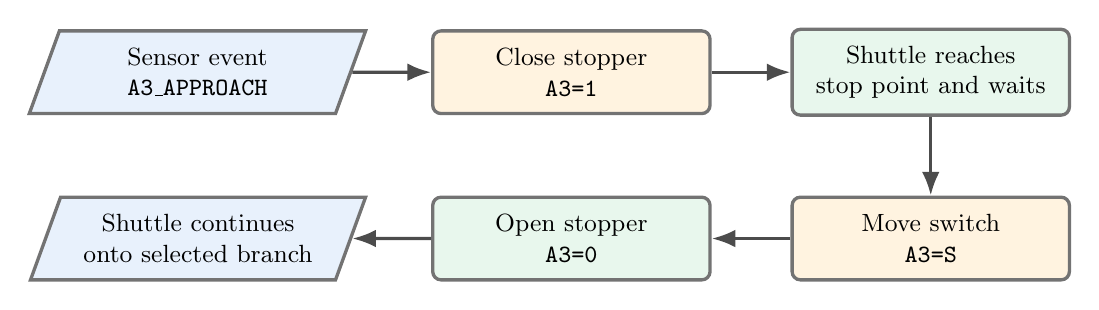
\begin{tikzpicture}[node distance=1.0cm and 1.0cm]
\node[flowio, fill=flowblue] (sensor) {Sensor event\\\texttt{A3\_APPROACH}};
\node[flowbox, fill=floworange, right=of sensor] (stop) {Close stopper\\\texttt{A3=1}};
\node[flowbox, fill=flowgreen, right=of stop] (wait) {Shuttle reaches\\stop point and waits};
\node[flowbox, fill=floworange, below=of wait] (switch) {Move switch\\\texttt{A3=S}};
\node[flowbox, fill=flowgreen, left=of switch] (release) {Open stopper\\\texttt{A3=0}};
\node[flowio, fill=flowblue, left=of release] (continue) {Shuttle continues\\onto selected branch};

\draw[flowarrow] (sensor) -- (stop);
\draw[flowarrow] (stop) -- (wait);
\draw[flowarrow] (wait) -- (switch);
\draw[flowarrow] (switch) -- (release);
\draw[flowarrow] (release) -- (continue);
\end{tikzpicture}}
\caption{Stopper-based switch workflow. The stopper and switch are separate
primitives: the stopper creates a safe waiting point, and the switch selects the
future route.}
\label{fig:stop-switch-release-flow}
\end{figure}

\section{Add shuttles during simulation}

After the node is already running, add a shuttle from a free slot:

\begin{lstlisting}[style=terminalcode]
ros2 topic pub --once /room_315/shuttle/add_cmd std_msgs/msg/String "{data: 'slot=3'}"
\end{lstlisting}

Add with a custom entity name and speed:

\begin{lstlisting}[style=terminalcode]
ros2 topic pub --once /room_315/shuttle/add_cmd std_msgs/msg/String "{data: 'entity=room315_shuttle_5 slot=4 speed=0.2'}"
\end{lstlisting}

If the requested slot is still occupied, the node rejects the command. This is
expected behavior. Wait until the current shuttle has moved away from the start
slot, or choose another free slot.

\section{Turn individual shuttles ON or OFF}

Turn one shuttle OFF:

\begin{lstlisting}[style=terminalcode]
ros2 topic pub --once /room_315/shuttle/control_cmd std_msgs/msg/String "{data: 'room315_shuttle_2=OFF'}"
\end{lstlisting}

Turn it ON again:

\begin{lstlisting}[style=terminalcode]
ros2 topic pub --once /room_315/shuttle/control_cmd std_msgs/msg/String "{data: 'room315_shuttle_2=ON'}"
\end{lstlisting}

Turn all shuttles OFF or ON:

\begin{lstlisting}[style=terminalcode]
ros2 topic pub --once /room_315/shuttle/control_cmd std_msgs/msg/String "{data: 'ALL=OFF'}"
ros2 topic pub --once /room_315/shuttle/control_cmd std_msgs/msg/String "{data: 'ALL=ON'}"
\end{lstlisting}

The state topic should show \texttt{enabled=false} and
\texttt{stopped\_by=DISABLED} for a disabled shuttle.

\section{Pose calibration controls}

The accepted CSV coordinates already include the calibration that was found
during testing. Normal operation should use default scale and offset values.
However, runtime calibration is still available for future alignment tests.

Start with temporary X and Y correction:

\begin{lstlisting}[style=terminalcode]
ros2 run mfja_robot_control_config room_315_kinematic_shuttle_node.py --ros-args \
  -p gazebo_world_name:=room_315_only \
  -p enable_gazebo_set_pose:=true \
  -p gazebo_entity_name:=room315_shuttle_1 \
  -p speed:=0.2 \
  -p gazebo_set_pose_rate_hz:=10.0 \
  -p pose_scale_x:=1.0 \
  -p pose_scale_y:=1.0 \
  -p pose_offset_x:=0.0 \
  -p pose_offset_y:=0.0 \
  -p pose_offset_z:=0.0
\end{lstlisting}

Change offset while the node is running:

\begin{lstlisting}[style=terminalcode]
ros2 topic pub --once /room_315/shuttle/pose_offset_cmd std_msgs/msg/String "{data: 'x=-0.02 y=0.01 z=0.00'}"
\end{lstlisting}

This should be used only for calibration experiments. Once the correct values
are known, the preferred method is to bake the correction into the CSV path data
and run the node with default calibration parameters.

\section{Validation commands}

Run preprocessing and validation:

\begin{lstlisting}[style=terminalcode]
cd /home/tiago/ALI_ros2_ws
source /opt/ros/jazzy/setup.bash
source install/setup.bash

ros2 run mfja_robot_control_config room_315_csv_preprocessor.py
ros2 run mfja_robot_control_config room_315_network_validator.py
ros2 run mfja_robot_control_config room_315_segment_plot.py
\end{lstlisting}

Expected validator result:

\begin{lstlisting}[style=terminalcode]
Status: PASS (0 warnings)
\end{lstlisting}

For the continuous path validator, the expected result is:

\begin{lstlisting}[style=terminalcode]
Validated continuous paths for 14 segments.
Status: PASS (0 warnings)
\end{lstlisting}

Generated files:

\begin{itemize}
\item normalized CSV output:
\codepath{mfja_robot_control_config/config/room_315_kinematics/normalized_segments};
\item segment summary:
\codepath{mfja_robot_control_config/config/room_315_kinematics/segment_summary.yaml};
\item validation report:
\codepath{mfja_robot_control_config/config/room_315_kinematics/validation_report.yaml};
\item continuous path report:
\codepath{mfja_robot_control_config/config/room_315_kinematics/continuous_path_report.yaml};
\item network plot:
\codepath{mfja_robot_control_config/config/room_315_kinematics/debug_plots/network_validation.png}.
\item continuous path comparison plot:
\codepath{mfja_robot_control_config/config/room_315_kinematics/debug_plots/continuous_path_validation.png}.
\end{itemize}

\section{Path backend selection}

Normal demos should use the continuous path backend:

\begin{lstlisting}[style=terminalcode]
-p path_backend:=cubic_hermite
\end{lstlisting}

The old CSV polyline backend is still available for comparison and debugging:

\begin{lstlisting}[style=terminalcode]
-p path_backend:=polyline
\end{lstlisting}

The recommended policy is to run with \texttt{cubic\_hermite} and keep
\texttt{polyline} as a reference. The validator compares these two backends, so
removing \texttt{polyline} would remove the easiest way to prove that the
continuous path did not drift away from the measured CSV data.

\section{Troubleshooting table}

\begin{longtable}{@{}p{0.33\textwidth}p{0.57\textwidth}@{}}
\toprule
Symptom & Most likely cause and action \\
\midrule
\endhead
\texttt{Gazebo set\_pose service is not ready yet} &
The bridge is missing, the world name is wrong, or Gazebo is not fully ready.
Run \texttt{ros2 service list | grep set\_pose} and make sure the shuttle node
uses the same \texttt{gazebo\_world\_name}. \\
\addlinespace
Shuttle does not appear in the full-floor world &
The node may still be using \texttt{room\_315\_only}. Start it with
\texttt{-p gazebo\_world\_name:=mfja\_3rd\_floor}. \\
\addlinespace
Switch moves visually but the route does not change &
The command was likely sent to the visual topic only. Send route commands to
\texttt{/room\_315/switch\_states}. \\
\addlinespace
Shuttle stops at a switch approach &
Check \texttt{stopped\_by} on the state topic. If it is a stopper name, release
that stopper with \texttt{/room\_315/stopper\_states}. \\
\addlinespace
Shuttle is waiting with \texttt{stopped\_by=DISABLED} &
It was turned OFF by \texttt{/room\_315/shuttle/control\_cmd}. Send
\texttt{room315\_shuttle\_N=ON}. \\
\addlinespace
Shuttle is waiting with \texttt{blocked\_by} set &
Collision avoidance is active. The named shuttle is too close. Move, stop, or
release shuttles so spacing becomes safe. \\
\addlinespace
Add command is rejected because a slot is occupied &
This is the current correct behavior. Wait until the slot is clear or choose
another slot. \\
\addlinespace
Add command for slot 5 is rejected &
Only four start slots exist in the current accepted configuration:
\texttt{1}, \texttt{2}, \texttt{3}, and \texttt{4}. \\
\addlinespace
Shuttle enters \texttt{FALLING} &
The current segment has no valid successor under the current switch state. Check
the routing table and current switch states. \\
\bottomrule
\end{longtable}

\chapter{What Was Built in This Phase}

This chapter summarizes the concrete engineering changes that define the
current version of the repository.

\section{Repository cleanup and package separation}

The repository was cleaned into a meta-repository shape. Root-level package
artifacts were removed or moved into the packages that own them. The current
structure separates:

\begin{itemize}
\item Gazebo descriptions and worlds;
\item launch entry points for Room 315 and the full floor;
\item shared robot and shuttle control configuration;
\item compatibility launch entry points;
\item repository-level documentation.
\end{itemize}

This makes the project easier to build with explicit \texttt{colcon} package
selection and prevents unrelated assets from being mixed at the root.

\section{Dynamic shuttle work removed from the current main path}

Earlier dynamic/contact-based shuttle experiments were removed from this branch
because they were not the accepted direction for the current phase. The current
approach is kinematic-first:

\begin{itemize}
\item validate CSV rail geometry offline;
\item validate explicit topology and switch routing;
\item run one-shuttle logic without Gazebo;
\item add ROS and Gazebo pose control;
\item add multiple shuttles, stoppers, sensors, and simple collision avoidance;
\item postpone contact dynamics, wheels, and rail contact physics.
\end{itemize}

This order reduces risk because path logic can be tested before physics
complexity is introduced.

\section{Room 315 rail graph and validation pipeline}

The rail network was split into directed CSV segments. The accepted segment
names are:

\begin{lstlisting}[style=terminalcode]
A1G A1S A2G A2S A3G A3S A4G A4S A12E A12I A14 A23 A34E A34I
\end{lstlisting}

The validation tools produce:

\begin{itemize}
\item normalized CSV files;
\item segment lengths;
\item duplicate-removal counts;
\item endpoint-to-anchor distances;
\item gap warnings above \texttt{0.05 m};
\item tangent mismatch warnings above \texttt{25 deg};
\item a debug plot with node labels and segment labels.
\end{itemize}

The latest expected result is a clean pass with no warnings.

\section{Continuous path backend added}

The shuttle geometry layer now supports parametrized path backends. The current
recommended runtime backend is \texttt{cubic\_hermite}. It turns calibrated CSV
points into a continuous arc-length path so the shuttle pose and yaw change more
smoothly through curves.

The original \texttt{polyline} backend remains available on purpose. It is the
reference backend used to compare against the measured CSV data. Keeping both
backends gives a safe workflow:

\begin{lstlisting}[style=terminalcode]
normal demos:        path_backend:=cubic_hermite
debug/reference use: path_backend:=polyline
\end{lstlisting}

The new validator produces
\codepath{mfja_robot_control_config/config/room_315_kinematics/continuous_path_report.yaml}
and
\codepath{mfja_robot_control_config/config/room_315_kinematics/debug_plots/continuous_path_validation.png}.
The current result is \texttt{PASS (0 warnings)}, with millimeter-level
deviation from the CSV polyline reference.

\section{Switches made independent and visible}

The shuttle route switch state is controlled by
\texttt{/room\_315/switch\_states}. Commands sent there update both the graph
routing state and the visual conveyor switch command topic. This gives one
operator command for logical and visual behavior.

The current logical switch states are \texttt{G} and \texttt{S}, matching the
segment suffixes in the network file. Historical aliases such as left/right or
specific visual names may exist in the visual layer, but the current route graph
uses \texttt{G}/\texttt{S} as the stable internal representation.

\section{Stopper primitive added before switches}

Independent binary stoppers were added before switches \texttt{A1},
\texttt{A2}, \texttt{A3}, and \texttt{A4}. This fills the workflow gap from the
meeting requirement:

\begin{lstlisting}[style=terminalcode]
sensor -> stop shuttle -> move switch -> unstop shuttle
\end{lstlisting}

The stopper primitive is intentionally separate from the switch primitive. A
stopper answers the question: should the shuttle wait before entering this
switch area? A switch answers the question: which route is selected?

\section{Sensor workflow added}

The sensor topic publishes approach events before a switch. This is not a full
hardware sensor simulation yet. It is a deterministic software sensor derived
from the shuttle arc length and the configured stop point. It is enough for the
teaching and testing workflow because it tells the operator:

\begin{itemize}
\item which shuttle is approaching;
\item which switch is ahead;
\item which stopper protects that switch;
\item how far the shuttle is from the stop point;
\item whether the stopper is currently open or closed.
\end{itemize}

\section{Per-shuttle control added}

Each shuttle can now be turned ON or OFF independently. This was added because
the system needs an operational primitive that can pause a specific shuttle
without stopping the entire node or deleting the model from Gazebo.

The OFF state is visible in the state payload as:

\begin{lstlisting}[style=terminalcode]
enabled: false
mode: WAITING
stopped_by: DISABLED
\end{lstlisting}

\section{Runtime shuttle addition with occupied-slot rejection}

The node can spawn or control additional shuttles during simulation. The
current accepted policy rejects a new shuttle if the requested start slot is
occupied. This differs from the earlier experimental behavior where repeated
slot use was allowed and collision avoidance handled the overlap later.

The current behavior is safer and easier to explain:

\begin{itemize}
\item valid slot and free space: add the shuttle;
\item valid slot but occupied: reject the command;
\item invalid slot: reject the command.
\end{itemize}

\section{Simple collision avoidance added}

The current collision behavior is a kinematic guard. It does not simulate
physical contact. Instead, it detects that another shuttle is within
\texttt{0.33 m}. If movement would cross into that unsafe distance, the node
reduces the step and leaves the moving shuttle waiting at the last safe pose.

This is enough for the current phase because the purpose is to prevent shuttles
from visually merging and to model the expected "stop when touching another
shuttle" behavior.

\section{Room-only and full-floor compatibility}

The same shuttle node works in both launch modes. The only important world
parameter changes are:

\begin{itemize}
\item Room-only world: \texttt{-p gazebo\_world\_name:=room\_315\_only};
\item full-floor world: \texttt{-p gazebo\_world\_name:=mfja\_3rd\_floor}.
\end{itemize}

The bridge, set-pose service, and spawn service all depend on that world name.
If the world name is wrong, the node can publish ROS pose topics but Gazebo will
not move the visible shuttle model.

\section{Shuttle mesh and pose alignment}

The shuttle STL was updated from the corrected model file. The important
practical lesson is that changing a mesh origin in CAD does not always produce
the expected model-frame behavior in Gazebo if the SDF visual, collision, or
link pose still applies an offset. For operational alignment, the accepted path
calibration was applied to the CSV path data, and the node also keeps runtime
pose calibration parameters for future tests.

The normal startup command should now run without custom scale or offset
parameters.

\chapter{Developer Notes for Future Work}

\section{Why stoppers are not blocks yet}

The current stopper implementation is a local stop primitive. It stops a
shuttle at a configured point before a switch. It does not yet reserve long
sections of track. Full block occupancy is a later feature. That future layer
should decide whether a shuttle is allowed to enter a block based on downstream
occupancy, route state, and possibly priority rules.

\section{Why collision avoidance is not full traffic control}

Collision avoidance only checks physical spacing between current shuttle poses.
It is reactive. It prevents overlap but does not plan traffic. A future block
system should be proactive: it should prevent a shuttle from entering a region
that will become unsafe later.

\section{Recommended next implementation phase}

The recommended next phase is:

\begin{enumerate}
\item keep the current four start slots unless new measured entry points are
accepted;
\item add named blocks to \texttt{rail\_network.yaml};
\item assign every rail segment to one or more blocks;
\item publish block occupancy in the state topic;
\item prevent shuttles from entering occupied protected blocks;
\item keep stoppers as the physical stop primitive before switches;
\item keep switch routing separate from stopper and block logic.
\end{enumerate}

This preserves the clean separation already established:

\begin{lstlisting}[style=terminalcode]
geometry -> topology -> routing -> stopper control -> block occupancy -> Gazebo pose output
\end{lstlisting}

\chapter{Conclusion}

The current repository is no longer just a static Gazebo map and no longer a
single-package experiment. It is a ROS~2 meta-repository with dedicated
description, control, bringup, and compatibility packages. The multi-robot
layer provides independent namespaced control for several robot families. The
Room 315 layer provides a kinematic-first shuttle system built on explicit rail
topology, switch routing, stoppers, sensor-style workflow events, runtime
spawning, and per-shuttle control.

The most important engineering result is separation of responsibilities:
geometry is stored in package-local assets, topology is stored in
\texttt{rail\_network.yaml}, robot deployment is stored in YAML registries,
runtime behavior is implemented in ROS~2 nodes, and the operator interface is
exposed through explicit topics. This makes the project testable phase by
phase, while avoiding premature contact-dynamics complexity.

\end{document}
